\chapter{successioni}
\label{ch:successioni}

Una \myemph{successione} in un insieme $X$ è una
funzione\footnote{%
Utilizziamo il grassetto per evidenziare il fatto
che $\vec a$ è una \emph{lista} (o vettore) di numeri.
Nella scrittura a mano non è possibile usare il grassetto, ma potremmo
sottolineare il nome della variabile scrivendo $\underline a$ invece che $\vec a$.
In alternativa si potrebbe scrivere $\stackrel{\rightarrow}a$ oppure evitare
qualunque distinzione e scrivere più semplicemente $a$.}
$\vec a\colon \NN \to X$.
L'insieme delle funzioni $\NN \to X$ viene usualmente indicato
con $X^\NN$ e potremmo dunque scrivere $\vec a \in X^\NN$. In effetti una successione $\vec a$ può essere interpretata
come una sequenza infinita di elementi di $X$:
\[
  \vec a = (a_0, a_1, a_2, \dots, a_n, \dots )
\]
dove si intende
\[
   a_n = \vec a(n).
\]
Le componenti $a_n$ si chiamano \emph{termini} della successione.
I numeri $n$ si chiamano, invece, \emph{indici}.
L'intera
successione $\vec a$ può essere indicata con $(a_n)_{n=0}^\infty$
oppure $(a_n)_n$ oppure,
più semplicemente, con $a_n$ quando sia chiaro che si intende l'intera
successione $\vec a$ e non un singolo termine della stessa.%
\footnote{In alcuni testi le successioni vengono indicate
con la notazione $\ENCLOSE{a_n}$ che però è fuorviante in quanto
una successione in $X$ non è semplicemente un sottoinsieme di $X$:
l'ordine in cui vengono presi gli elementi è rilevante.}

Per noi il caso più interessante sarà quello delle \emph{successioni reali}
$a_n\in \RR$ cioè il caso $X=\RR$. Considereremo però anche il caso di
\emph{successioni complesse} $a_n\in \CC$ (dunque $X=\CC$) perché questo
potrà essere utile in alcune situazioni.

Le successioni vengono usualmente
considerate nei procedimenti di approssimazione.
Spesso infatti siamo interessati a capire qual è il numero (se esiste) a cui
la successione si avvicina al crescere di $n$.

\begin{definition}[successione convergente]
\mymark{***}
Diremo che una successione $a_n\in \RR$ converge
\mymargin{convergenza}
\index{successione!convergente}
ad un numero $\ell \in \RR$
e scriveremo:
\[
  a_n \to \ell \qquad\text{(per $n\to +\infty$)}
  \mymargin{$a_n\to \ell$}
\]
se scelto comunque un errore $\eps>0$ ogni termine della successione,
da un certo punto in poi, si trova a distanza inferiore di $\eps$
dal punto limite $\ell$. Formalmente:
\begin{equation}\label{eq:limite_successione}
\forall \eps>0\colon \exists N\in\NN \colon \forall n\in \NN\colon
n>N \implies \abs{a_n - \ell}
< \eps.
\end{equation}
Il valore $\ell$ verrà in tal caso chiamato \emph{limite} della successione.

La stessa definizione è valida per le successioni complesse
$a_n \in \CC$ dove il simbolo $\abs{\cdot}$ rappresenta il modulo complesso
invece che il valore assoluto. Si ottiene che $a_n\to \ell\in \CC$ se e solo se
$\abs{a_n-\ell}\to 0$ (si osservi che $\abs{a_n-\ell}$ è una successione reale).
\end{definition}

\begin{example}
La successione $a_n = \frac{n}{n+1}$ converge a $\ell=1$:
\[
  \frac{n}{n+1}\to 1 \qquad \text{per $n\to +\infty$}.
\]
\end{example}
%
Possiamo intuitivamente capire che la successione
$a_n = \frac{n}{n+1}$
tende a $1$ scrivendone i primi valori:
\begin{center}
\begin{tabular}{l|rrrrrrrrrrr}
$n$ & $0$ & $1$ & $2$ & $3$ & $4$ & $5$ & $6$ & $7$ & $8$ & $9$ & $\dots$ \\ \hline
$a_n $ \rule{0pt}{3ex} & $0$ &
$ \frac{1}{2} $ &
$ \frac{2}{3} $ &
$ \frac{3}{4} $ &
$ \frac{4}{5} $ &
$ \frac{5}{6} $ &
$ \frac{6}{7} $ &
$ \frac{7}{8} $ &
$ \frac{8}{9} $ &
$ \frac{9}{10} $ &
$ \dots $
\end{tabular}
\end{center}
Vogliamo però dare una dimostrazione formale.
%
\begin{proof}
Dato $\eps>0$ ci chiediamo quali siano gli indici $n$
per i quali risulta $\abs{a_n -1}<\eps$ e troviamo
che devono valere due disequazioni:
\[
  1- \eps < \frac{n}{n+1} < 1+\eps.
\]
Facilmente possiamo osservare che $n/(n+1)<1$ per ogni $n$, dunque
la seconda disequazione è sempre verificata. La prima disequazione
si riconduce a
\[
 n + 1 > \frac{1}{\eps}.
\]
Dunque qualunque sia $\eps>0$, scelto $N = \lceil 1 / \eps\rceil$
sappiamo che per ogni $n>N$
si ha $n+1 > n > N \ge \frac{1}{\eps}$ e quindi $1-\eps < a_n$.
Inoltre la disuguaglianza $a_n < 1 < 1+\eps$ è verificata per ogni $n$.
Abbiamo quindi verificato che vale la condizione che definisce
la convergenza.
\end{proof}

\begin{exercise}
Una successione complessa $z_n\in \CC$ potrà essere scritta
nella forma $z_n = x_n + i y_n$ dove $x_n$ e $y_n$ sono successioni
reali. Si può allora verificare che $z_n\to z$ per $z\in \CC$ se e solo se
$x_n\to x$ e $y_n\to y$ dove $z=x+ iy$ con $x,y\in \RR$.
\end{exercise}

Le successioni convergenti sono quelle che approssimano un
certo numero finito.
Vogliamo ora catturare l'idea di successioni che vanno verso i
punti all'infinito.

\begin{definition}[successione divergente]
\mymark{***}
\mymargin{divergente}
\index{successione!divergente}
Una successione $a_n\in \RR$ si dice avere limite $+\infty$
o divergere a $+\infty$
\mymargin{$a_n\to +\infty$}
\[
  a_n \to +\infty \qquad\text{(per $n\to +\infty$)}
\]
se comunque si scelga un numero reale, anche molto grande,
ogni termine della successione, da un certo punto in poi,
risulta essere maggiore di tale numero scelto. Formalmente
\begin{equation}\label{eq:limite_infinito_successione}
  \forall M\in \RR\colon \exists N\in \NN \colon \forall n\in \NN\colon
  n>N \implies a_n >M.
\end{equation}
Definizione analoga si ha per il limite $-\infty$. Scriveremo
\mymargin{$a_n\to -\infty$}
\[
  a_n \to -\infty \qquad \text{(per $n\to +\infty$)}
\]
se $-a_n\to +\infty$ ovvero se
\begin{equation}\label{eq:limite_meno_infinito_successione}
  \forall M\in \RR\colon \exists N\in \NN \colon \forall n\in \NN\colon
  n>N\implies a_n < -M.
\end{equation}

Un successione reale $a_n$ si dirà essere \emph{divergente}
se $a_n\to +\infty$ o $a_n\to -\infty$.

Se invece $a_n$ è una successione complessa diremo che $a_n$ diverge e scriveremo
$a_n \to \infty$
se
\[
  \forall M\in \RR\colon \exists N \in \NN \colon \forall n\in \NN \colon
  n>N \implies \abs{a_n} > M
\]
che, è equivalente a richiedere che $\abs{a_n}\to +\infty$
(si osservi infatti che $\abs{a_n}$ è una successione reale).
\end{definition}

\begin{example}
Si ha
\[
  1000-n^2 \to -\infty.
\]
\end{example}
%
\begin{proof}
Per dimostrare che $1000-n^2\to -\infty$ sarà
necessario trovare per ogni $M\in \RR$
dei valori di $n$ per i quali si abbia $1000-n^2 < -M$.
Questo avviene se $n^2 > 1000 + M$. Visto che per ogni $n\in \NN$
si ha $n^2 \ge n$ (verificare!) sappiamo che se $n> 1000+M$ allora
anche $n^2 > 1000+M$. Dunque per ogni $M$ sarà sufficiente considerare
un numero intero $N \ge 1000 + M$
(ad esempio si potrebbe scegliere $N = \max\ENCLOSE{0, \lceil 1000 + M\rceil}$)
cosicché per ogni $n>N$ si avrebbe:
\[
 a_n = 1000 - n^2 \le 1000 - n < 1000 - N \le 1000 - (1000  + M) = -M
\]
come richiesto dalla definizione di limite $-\infty$.
\end{proof}

\begin{definition}[carattere di una successione]
\mymark{***}
Sia $a_n$ una successione a valori reali o complessi.
Se $a_n$ ammette limite (finito o infinito)
diremo che la successione $a_n$ è \emph{regolare}.
\index{successione!regolare}%
\index{regolare!successione}%
\mynote{successione regolare}%
Se $a_n$ non ammette limite
si dice anche che $a_n$ è \emph{irregolare}
\index{successione!irregolare}%
o \emph{indeterminata}
\mynote{successione indeterminata}%
\index{successione!indeterminata}%
(si intende che è indeterminato il suo limite!)
Abbiamo dunque le seguenti alternative
\begin{enumerate}
 \item la successione è convergente (ha limite finito);
 \item la successione è divergente (ha limite infinito);
 \item la successione è indeterminata (non ha limite).
\end{enumerate}
Determinare il \emph{carattere}
\mynote{carattere di una successione}%
\index{carattere!di una successione}%
di una successione
significa specificare a quale delle tre categorie appartiene.
\end{definition}

Si faccia attenzione al fatto che una successione $a_n\in \RR \subset \CC$
può essere interpretata sia come successione reale che come successione complessa.
Le condizioni di convergenza in $\RR$ o $\CC$ sono allora equivalenti. Ma
se $a_n \to \infty$ (in $\bar \CC$) significa che $\abs{a_n}\to +\infty$
e può capitare che $a_n$ non abbia limite né $+\infty$
né $-\infty$ in quanto potrebbe frequentemente cambiare di segno
(un esempio è $a_n = (-n)^n$).
In alcuni testi si usa il simbolo $\pm \infty$ per indicare
il limite $\infty$ nel contesto dei numeri reali. Si faccia però
attenzione che se consideriamo come possibili valore di un limite
sia $\pm\infty$ che $+\infty$ e $-\infty$ non si avrà più l'unicità
del limite in quanto una successione che tende a $+\infty$
tende anche a $\pm \infty$.

\begin{theorem}[unicità del limite]
\mymargin{unicità del limite}%
\index{limite!unicità}%
\index{unicità!del limite}%
Sia $a_n$ una successione a valori reali e siano $\ell_1,\ell_2\in \bar \RR$
tali che
\[
  a_n \to \ell_1, \qquad
  a_n \to \ell_2.
\]
Allora si ha $\ell_1=\ell_2$ (il limite, se esiste, è unico).
Lo stesso vale per le successioni a valori complessi che hanno limite
$\ell_1, \ell_2 \in \bar \CC$.
\end{theorem}
%
\begin{proof}
Supponiamo per assurdo che sia $\ell_1\neq \ell_2$.
Senza perdita di generalità possiamo anzi supporre
che sia $\ell_2 > \ell_1$. Ma allora certamente
esiste un numero $M\in \RR$ tale che $\ell_1 < M < \ell_2$.
Ora consideriamo la condizione $a_n\to \ell_1$.
Se $\ell_1=-\infty$ sappiamo che esiste $N_1\in\NN$
tale che per ogni $n> N_1$ si ha $a_n < M$.
Se $\ell_1\in \RR$ scegliamo $\eps = M-\ell_1$
cosicché dalla definizione di limite otteniamo comunque
che esiste $N_1\in \NN$ per cui per ogni $n>N_1$ si
ha $a_n < \ell_1+\eps = M$. Chiaramente non può essere
$\ell_1=+\infty$ in quanto abbiamo supposto che fosse
$\ell_1 < \ell_2$.

In maniera analoga dalla condizione $a_n\to \ell_2$
sia che $\ell_2$ sia finito sia che sia infinito
possiamo affermare che esiste un $N_2\in \NN$ tale
che per ogni $n>N_2$ si ha $a_n > M$.

Dunque, posto $N=\max\ENCLOSE{N_1,N_2}$ si ha,
per ogni $n>N$, $a_n < M < a_n$ che è palesemente assurdo.

Nel caso $a_n\in \CC$ consideriamo innanzitutto
il caso $\ell_1,\ell_2 \in \CC$. In questo
caso scegliamo $\eps = \frac{\abs{\ell_1-\ell_2}}{2}$.
Se per assurdo fosse $\ell_1\neq \ell_2$ avremmo $\eps>0$
e dunque dalle condizioni $a_n\to \ell_1$
e $a_n \to \ell_2$ troveremmo $N_1$ e $N_2$
tali che per $n>N_1$ si abbia $\abs{a_n-\ell_1}<\eps$
e per $n>N_2$ si abbia $\abs{a_n -\ell_2}<\eps$. Ma allora
per $n>\max\ENCLOSE{N_1,N_2}$ si avrebbe
\[
  2\eps
  = \abs{\ell_1-\ell_2}
  \le \abs{\ell_1-a_n} + \abs{a_n-\ell_2}
  < \eps + \eps
\]
che è assurdo!

Se invece fosse $\ell_1\in \CC$ e $\ell_2=\infty$
fissato $\eps=1$ esisterebbe $N_1\in \NN$
tale che $\abs{a_n-\ell_1}<
\eps$ per $n>N_1$ e fissato $M=\abs{\ell_1}+\eps$
esisterebbe $N_2\in \NN$ tale che $\abs{a_n} > M$ per $n>N_2$.
Avremmo allora che per $n>\max\ENCLOSE{N_1,N_2}$ si avrebbe
\[
  M
  <\abs{a_n}
  \le \abs{a_n-\ell_1}+\abs{\ell_1}
  \le \eps + \abs{\ell_1} = M
\]
che è pure assurdo.
\end{proof}

Osserviamo che non è detto che un limite esista, come si vede dal seguente esempio.

\begin{example}
Sia $a_n = (-1)^n$. Non esiste $\ell \in \bar \RR$
tale che $a_n \to \ell$.
\end{example}
\begin{proof}
Supponiamo per assurdo che si abbia $a_n\to \ell\in \bar \RR$.
Se fosse $\ell=+\infty$ mettendo $M=0$ nella definizione~\eqref{eq:limite_infinito_successione}
troveremmo che esiste $N\in \NN$ tale che per ogni $n>N$
si abbia $a_n>0$. Questo è assurdo in quanto sappiamo che se
$n$ è dispari si ha $a_n = (-1)^n = -1$.
Se fosse $\ell\in[0,+\infty)$ scegliendo $\eps=\frac 1 2$  nella definizione~\eqref{eq:limite_successione} troveremmo che
esiste $N\in \NN$ tale che per ogni $n>N$ si abbia $a_n > \ell-\eps \ge -\frac 1 2$. Anche questo è assurdo come nel caso precedente.

Se fosse $\ell=-\infty$ oppure $\ell\in (-\infty,0)$ si ragiona
in maniera: dalla definizione di limite si scopre che da un certo punto
in poi la successione deve assumere valori negativi o comunque inferiori a $\frac 1 2$ e questo contrasta con il fatto che la
successione assume il valore $1$ su tutti i termini di indice pari.
\end{proof}

Abbiamo dunque osservato che in generale il limite di una successione può
non esistere ma se esiste è unico.
Questo ci permette di definire l'operatore $\lim$
(limite) che associa ad ogni successione regolare
il suo (unico) limite in $\bar \RR$
(o in $\bar \CC$ per le sottosuccessioni complesse).
Dunque se $a_n \to \ell$ scriveremo
\mymargin{$\lim a_n$}
\[
  \lim a_n = \ell.
\]
Per evidenziare il fatto che nella precedente formula
$n$ compare come variabile muta potremo scrivere
in maniera più espressiva
\[
   \lim_{n\to+\infty} a_n = \ell
   \qquad\text{oppure}\qquad
   \lim_n a_n = \ell.
\]

\section{definizione topologica di limite}

Volendo esprimere il concetto di limite in maniera uniforme
(senza dover distinguere limiti finiti e infiniti) possiamo
rendere la definizione un poco più astratta introducendo il concetto
di \emph{intorno}.
La condizione $\abs{a_n - \ell}< \eps$ può essere scritta in
modo equivalente come
$a_n \in (\ell-\eps, \ell+\eps)$. L'insieme $B_\eps(\ell) = (\ell-\eps, \ell+\eps)$
si chiama \myemph{intorno simmetrico} di raggio $\eps$ centrato in $\ell$.
Possiamo quindi considerare la famiglia
di tutti questi intorni del punto $\ell$:
\[
 \B_\ell = \ENCLOSE{B_\eps(\ell)\colon \eps>0 }.
\]
Questa famiglia di insiemi si chiama \myemph{base di intorni} del punto $\ell$.
La definizione
di limite finito si può dunque riscrivere così:
\begin{equation}\label{eq:034333}
  a_n\to \ell
  \qquad \iff \qquad
  \forall B \in \B_\ell\colon \exists N\in \NN\colon \forall n>N\colon a_n\in B.
\end{equation}
Il vantaggio di questa \emph{astrazione} è che ora possiamo definire
gli intorni di $+\infty$ e di $-\infty$ nel modo seguente:
\begin{align*}
  \B_{+\infty} &= \ENCLOSE{ (M,+\infty]\colon M\in \RR}\\
  \B_{-\infty} &= \ENCLOSE{ [-\infty, -M)\colon M \in \RR}
\end{align*}
e la definizione~\eqref{eq:034333} risulta valida anche nel
caso in cui $\ell$ sia infinito.
Potremmo in realtà andare oltre, osservando che la condizione
$\exists N\in \NN \colon \forall n>N$ può essere rimpiazzata
da $\exists U\in \mathcal B_{+\infty}\colon \forall n\in U$
arrivando quindi alla definizione equivalente \
\[
\forall B\in \mathcal B_l\colon \exists U\in \mathcal B_{+\infty}\colon
\forall n\in \NN \colon n\in U \implies a_n\in B.
\]
Se ora ci ricordiamo che $a_n = \vec a(n)$ con $\vec a\colon \NN \to \RR$
possiamo infine arrivare alla seguente definizione equivalente
\[
\forall B\in \mathcal B_l\colon \exists U\in \mathcal B_{+\infty}\colon
\vec a(U)\subset B.
\]

In generale se per ogni punto $x$ di un insieme $X$ specifichiamo quale
sia una base di intorni $\B_x$ di $x$, potremo definire i limiti delle successioni
a valori in $X$.
Nel caso $X=\CC$ gli intorni di un punto $z_0\in \CC$ sono gli insiemi
(palle) della forma:
\[
  B_\rho(z_0) = \ENCLOSE{z\in \CC \colon \abs{z-z_0}<\rho}
\]
e dunque $\B_{z} = \ENCLOSE{B_\rho(z)\colon \rho>0}$. Se $X=\bar \CC$ dovremo
definire anche gli intorni di $\infty$:
\[
  \B_\infty = \ENCLOSE{ \ENCLOSE{z\in \CC\colon \abs{z}>\rho} \colon \rho>0}.
\]
Con queste definizioni la condizione~\eqref{eq:034333} è valida
anche per le successioni complesse.

\section{proprietà frequenti e definitive}

\begin{definition}[proprietà frequenti e definitive]
Sia $P(n)$ un predicato dipendente da un numero naturale $n\in \NN$.
Diremo che $P(n)$ vale \myemph{definitivamente} (in $n$) se
\[
  \exists N\in \NN \colon \forall n>N\colon P(n).
\]
Diremo che $P(n)$ vale \myemph{frequentemente} (in $n$) se
\[
  \forall N\in \NN \colon \exists n>N \colon P(n).
\]
\end{definition}

Chiaramente se una proprietà vale definitivamente vale anche frequentemente.
E dire che vale frequentemente è equivalente a dire che
l'insieme $\ENCLOSE{n\in \NN\colon P(n)}$ è infinito (cioè la proprietà vale per infiniti
valori di $n\in \NN$).

Le due proprietà sono complementari nel senso che vale la seguente
relazione:
\[
  \text{non frequentemente $P(n)$} \iff
  \text{definitivamente non $P(n)$}
\]

Se due proprietà $P(n)$ e $Q(n)$ valgono definitivamente allora anche
$P(n)\land Q(n)$ vale definitivamente. Se invece valgono entrambe
frequentemente allora anche $P(n) \lor Q(n)$ vale frequentemente.

\begin{example}
La proprietà
\[
  \text{$n$ è un numero pari}
\]
vale frequentemente in $n$. La proprietà
\[
 \text{$n! > 2^n$}
\]
vale definitivamente in $n$.
\end{example}

La definizione di limite $a_n \to \ell$ potrebbe quindi enunciarsi così:
per ogni intorno $B$ di $\ell$ si ha $a_n\in B$ definitivamente.
E la sua negazione è: esiste un intorno $B$ di $\ell$ per cui
frequentemente $a_n\not\in B$.

\begin{comment}
%%
%% unicita del limite usando le definizioni topologiche
%% tramite proprieta' di separazione
%%
\begin{theorem}[proprietà di separazione di $\bar \RR$ e $\bar \CC$]
\label{th:separazione_R_e_C}
Punti distinti $\ell_1 \neq \ell_2$ in $\bar \RR$ o in $\bar \CC$
ammettono intorni disgiunti $B_1 \in \B_{\ell_1}$, $B_2\in \B_{\ell_2}$,
$B_1 \cap B_2 = \emptyset$.
\end{theorem}
\begin{proof}
Consideriamo innanzitutto $\ell_1,\ell_2\in \bar \RR$.
Se $\ell_1$ ed $\ell_2$ sono entrambi finiti, è sufficiente
considerare $\eps = \abs{\ell_2-\ell_1}/2$.
Dall'interpretazione
geometrica risulta chiaro
che gli intorni $B_1=B_\eps(\ell_1)$ e
$B_2=B_\eps(\ell_2)$
sono disgiunti. Algebricamente questo si ottiene applicando
opportunamente la disuguaglianza triangolare per il valore assoluto.

Se $\ell_1$ ed $\ell_2$ sono entrambi infiniti e sono diversi,
possiamo supporre $\ell_1=-\infty$ e $\ell_2=+\infty$. In tal caso gli
intorni $B_1= [-\infty,0)$ e $B_2=(0,+\infty]$ sono disgiunti.
Se $\ell_1$ è finito e $\ell_2 = +\infty$, basterà prendere
$B_1 = (\ell_1-1, \ell_1+1)$ ed $B_2 = (\ell_1+1,+\infty]$ per avere due
intorni disgiunti. Analogamente si procederà nel caso $\ell_2=-\infty$.

Per $\ell_1,\ell_2 \in \bar \CC$ la dimostrazione si fa in maniera del tutto analoga:
per due punti in $\CC$ si può prendere come $\eps=\abs{\ell_2-\ell_1}/2$
metà della distanza tra i due
punti: la disuguaglianza triangolare del modulo garantirà che
$B_\rho(\ell_1)\cap B_\rho(\ell_2)=\emptyset$.
 Se uno dei due punti è $\ell_2=+\infty$ e l'altro è $\ell_1\in \CC$
si potrà prendere $B_1(\ell_1)$  come intorno di raggio unitario di $\ell_2$ e
$\ENCLOSE{z\colon \abs{z}>\abs{\ell_2}+1 }$
come intorno del punto $\infty$. La disuguaglianza triangolare ci assicura
che questi due intorni sono disgiunti, come ovvio da una interpretazione geometrica.
\end{proof}
%
%
\begin{theorem}[unicità del limite]
\mymargin{unicità del limite}
Sia $a_n$ una successione a valori reali e siano $\ell_1,\ell_2\in \bar \RR$
tali che
\[
  a_n \to \ell_1, \qquad
  a_n \to \ell_2.
\]
Allora si ha $\ell_1=\ell_2$ (il limite, se esiste, è unico).
Lo stesso vale per le successioni a valori complessi che hanno limite
$\ell_1, \ell_2 \in \bar \CC$.
\end{theorem}
%
\begin{proof}
Questo risultato discende direttamente dalla proprietà enunciata nel
teorema~\ref{th:separazione_R_e_C}. Se una successione avesse due limiti
diversi allora potrei trovare due intorni disgiunti dei due punti limite
e la definizione di limite mi direbbe che la successione deve stare
definitivamente in ognuno dei due intorni. Questo è impossibile.
\end{proof}
%%
%%
\end{comment}

\section{criteri di confronto}

\begin{theorem}[criteri di confronto]
\label{th:confronto_successioni}%
\index{teorema!del confronto (successioni)}%
\index{limite!successione!confronto}%
\index{teorema!dei due carabinieri (successioni)}%
\mymark{***}%
Siano $a_n$, $b_n$ e $c_n$ successioni a valori reali%
\footnote{Non è possibile fare confronti tra valori complessi, visto che
sui numeri complessi non abbiamo un ordinamento}.
\mymargin{confronto tra limiti}
\begin{enumerate}
\item
Se per ogni $n\in \NN$ si ha
\[
a_n \le b_n
\]
e se entrambe le successioni ammettono limite: $a_n \to a$ e $b_n \to b$
allora
\[
a \le b.
\]

\item
Se per ogni $n$ si ha:
\[
a_n \le b_n
\]
e se $a_n\to +\infty$ allora anche $b_n \to +\infty$.
Viceversa se $a_n \le b_n$ e $b_n \to -\infty$ allora anche $a_n \to -\infty$.

\item
(teorema dei carabinieri)
\mynote{teorema dei carabinieri}
\index{teorema!dei carabinieri}
Se per ogni $n$ vale
\[
a_n \le b_n \le c_n
\]
 e se le due
successioni $a_n$ e $c_n$ hanno lo stesso limite: $a_n \to \ell$ e $c_n\to \ell$
allora anche $b_n \to \ell$.
\end{enumerate}
\end{theorem}
%
\begin{proof}
\mymark{**}
\begin{enumerate}
\item
Se per assurdo fosse $a > b$ esisterebbero degli intorni disgiunti $B_a\in \B_a$
e $B_b \in \B_b$.
Inoltre si avrebbe $B_a > B_b$ (cioè: ogni punto di $B_a$ sarebbe maggiore
di ogni punto di $B_b$) visto che $a>b$.
Ma, dalla definizione di limite,
si dovrebbe avere che definitivamente $a_n\in B_a$ e $b_n\in B_b$ il che
è assurdo se $a_n\le b_n$ e $B_a > B_b$.

\item
Se $a_n \to +\infty$ per ogni $M\in \RR$
si ha $a_n > M$ definitivamente.
Ma se $b_n>a_n$ si ha anche $b_n >M$.
Questo è vero per ogni $M\in \RR$ e quindi
si ottiene la definizione di limite $b_n \to +\infty$.
Dimostrazione analoga si ottiene nel caso $b_n \to -\infty$.

\item
Se $a_n$ e $c_n$ hanno lo stesso limite $\ell$ significa che per ogni
$B \in \B_\ell$
si ha $a_n\in B$ e $c_n\in B$ definitivamente.
Ma allora anche $b_n\in B$ definitivamente. Essendo questo
vero per ogni $B\in \B_\ell$ si ottiene la definizione di limite
$b_n \to \ell$.
\end{enumerate}
\end{proof}

\begin{theorem}[successioni che differiscono su un numero finito di termini]
\mymark{**}%
\mynote{successioni definitivamente uguali}%
\index{successioni!che differiscono su un numero finito di termini}%
\index{successioni!definitivamente uguali}%
Se $a_n$ e $b_n$ sono due successioni
che differiscono solamente per un numero finito di termini
(significa l'insieme $\ENCLOSE{n\in \NN\colon a_n \neq b_n}$ è finito)
allora $a_n$ e $b_n$ hanno lo stesso carattere e se non
sono indeterminate hanno lo stesso limite.
\end{theorem}
%
\begin{proof}
Due successioni che differiscono su un numero finito
di termini sono definitivamente uguali.
Avere limite $\ell$ significa che per ogni $B$ intorno di $\ell$
la successione sta definitivamente in $B$ e dunque la condizione
è equivalente se le successioni sono definitivamente uguali.
Significa che hanno lo stesso carattere e lo stesso limite.
\end{proof}

Il teorema precedente è molto utile perché ci permette di applicare
i criteri di confronto anche nel caso in cui le ipotesi siano violate
su un numero finito di termini, come nel seguente esempio.

\begin{example}
Sapendo che la successione $a_n = n$ tende a $+\infty$ dimostrare
che anche la successione $b_n = n^2-10$ tende a $+\infty$.
\end{example}
%
\begin{proof}
E' sufficiente osservare che $n^2-10 > n$ se $n\ge 4$ infatti
se $n\ge 4$ si ha
\[
n^2 - 10 \ge 4 n -10 = n + 3n - 10 \ge n + 12 -10 \ge n+2 > n.
\]
Dunque se consideriamo la successione $c_n$ ottenuta da $b_n$
modificando i primi quattro termini (ponendo ad esempio $c_0 = a_0$,
$c_1=a_1$, $c_2=a_2$ e $c_3=a_3$) si ottiene $c_n\ge a_n$ per ogni $n$.
Ma allora $c_n \to +\infty$ (per confronto con $a_n$) ma visto che
$b_n$ differisce da $c_n$ solo nei primi 4 termini anche $b_n\to +\infty$.
\end{proof}

Il teorema precedente garantisce inoltre
che per quanto riguarda lo studio del limite possiamo considerare
successioni che siano definite solamente da un certo indice in poi.
Ad esempio è molto frequente considerare successioni il cui primo indice sia
$n=1$ invece che $n=0$. Questo non cambia nulla per quanto riguarda il limite
della successione.

\begin{example}
La successione $a_n = 1/n$ è definita per $n\in \NN$ ma $n\neq 0$.
Ciò non toglie che possiamo studiarne il limite come qualunque altra
successione. Per evidenziare il fatto che il primo indice è $n=1$
si potrà usare la notazione $(a_n)_{n=1}^\infty$.
Per la cronaca: $1/n \to 0$.
\end{example}


\begin{corollary}[permanenza del segno]
\mymark{***}%
\mynote{permanenza del segno}%
\index{permanenza del segno (successioni)}%
\index{teorema!della permanenza del segno (successioni)}%
Sia $a_n$ una successione e $c\in \RR$.

Se per ogni $n\in \NN$ si ha $a_n \ge c$ e se $a_n$ ha limite $\ell \in \bar \RR$
allora $\ell \ge c$.
In particolare se una successione regolare ha tutti i valori non negativi,
allora il limite è non negativo.

Viceversa, se
$a_n \to a > c$ allora si avrà $a_n>c$ definitivamente
(cioè per tutti gli $n\in \NN$ tranne al più un numero finito
di termini).
Risultato analogo vale se $a_n \to a < c$: si avrà
definitivamente $a_n < c$.
\end{corollary}
%
\begin{proof}
\mymark{**}
Per la prima parte
è sufficiente considerare la successione costante $c_n = c$
cosicché si ha $c_n \le a_n$ per ogni $n$. Ma ovviamente
la successione $c_n$ ha limite $c$ e dunque,
per confronto (teorema~\ref{th:confronto_successioni}),
deve essere $c\le \ell$.

Seconda parte. Se $a>c$ e $a\in \RR$
per definizione di limite scelto $\eps = a-c$ esiste $N$
tale che per ogni $n>N$ si ha $a_n > a-\eps = c$.
Dunque solo per un numero finito di termini
(quelli con indice inferiore a $N$)
si può avere $a_n \le c$.
Se $a=+\infty$ il ragionamento
si ripete a maggior ragione sapendo che esiste $N$
tale che $a_n>c$ per $n>N$.
Dimostrazione analoga (invertendo opportunamente le disuguaglianze)
si ottiene per $a<c$.
\end{proof}

Si presti molta attenzione al fatto che se $a_n$ è a termini positivi
non è detto che il limite sia positivo, possiamo solo affermare
che non è negativo. Ad esempio $a_n = \frac{1}{n+1}>0$
ma $a_n \to 0$ (verificare!).
In generale se una successione ha valori in un intervallo il suo limite,
se esiste, deve essere un punto del corrispondente intervallo chiuso.

Se una successione ha limite $0$ può avere infiniti termini
positivi e infiniti termini negativi, come nel caso
della successione $a_n = 1/(-2)^n$.

\section{limitatezza}

Data una successione $a_n$ potremo considerare l'\emph{insieme
dei suoi valori}: $\ENCLOSE{a_n\colon n\in \NN}$.
Si tratta dell'immagine della funzione $n\mapsto a_n$
e a volte si chiama \myemph{supporto} della successione.
Si faccia attenzione al fatto che l'insieme dei valori
non descrive completamente la successione perché
viene persa l'informazione sull'ordine in cui vengono elencati
i termini della successione e sulla loro molteplicità (ogni valore
potrebbe essere assunto su molti indici diversi). Ad esempio
l'insieme dei valori della successione $a_n = (-1)^n$ è l'insieme $\ENCLOSE{-1, 1}$. Ma anche la successione
\[
 b_n = \begin{cases}
   -1 & \text{se $n\le 42$}\\
   1  & \text{altrimenti}
 \end{cases}
\]
ha lo stesso insieme dei valori.
Si osservi però
che la prima successione è indeterminata
mentre la seconda è convergente (verificare!).

Ricordandoci che una successione reale $a_n$ non è altro che
una funzione $\vec a \colon \NN \to \RR$
ha senso applicare alle successioni gli operatori
$\sup$, $\inf$, $\max$ e $\min$
(si veda la definizione~\ref{def:funzione_limitata}).
Queste operazioni potrebbero essere sensibili anche ai primi termini della
successione (a differenza dell'operazione di limite) dunque potrebbe
essere necessario, per chiarezza, specificare qual è il primo indice
da cui si intende cominciare a considerare i valori. Ad esempio
se la successione $a_n$ è definita sui naturali tranne lo zero
si avrà:
\[
  \sup a_n = \sup_{n=1}^\infty a_n = \sup\ENCLOSE{a_n \colon n \in \NN, n \ge 1}.
\]

\begin{example}
Si consideri $a_n = \frac{1}{n+1}$ definita per $n\in \NN$.
Allora
\[
  \sup a_n = \max a_n = 1, \qquad
  \inf a_n = 0, \qquad \text{non esiste }\min a_n.
\]
\end{example}
\begin{proof}
Per ogni $n \in \NN$ si ha $n+1\ge 1$ e quindi $a_n = 1/(n+1) \le 1$.
Visto poi che $a_0 = 1$ si ottiene immediatamente che $\max a_n = 1$
e di conseguenza $\sup a_n = 1$.

Per verificare che $\inf a_n = 0$ dobbiamo verificare innanzitutto
che $0$ è minorante, e questo è vero in quanto $a_n = 1/(n+1)> 0$ essendo $n+1\ge 1 \ge 0$.
Inoltre dobbiamo verificare che per ogni $\eps >0$ esiste $n\in \NN$ tale
che $a_n < 0 + \eps = \eps$. Questo succede se $1/(n+1) < \eps$ ovvero
se $n > 1/\eps -1$ ad esempio per $n=\lceil 1/\eps\rceil$.
Abbiamo dunque verificato che $\inf a_n = 0$.
Il minimo di $a_n$ non esiste perché se esistesse dovrebbe essere uguale
all'estremo inferiore cioè dovrebbe essere $0$. Ma questo è impossibile
perché per ogni $n\in \NN$ si ha $a_n = 1/(n+1)\neq 0$.
\end{proof}

Sempre considerando la definizione~\ref{def:funzione_limitata}
una successione $a_n$ risulta essere
\emph{superiormente limitata}
\mymargin{successione limitata}%
\index{successione!superiormente limitata}%
se $\sup a_n < +\infty$
ovvero:
\[
  \exists M\in \RR\colon \forall n \in \NN\colon a_n \le M.
\]
In maniera analoga si dice che la successione $a_n$ è
\emph{inferiormente limitata}
\index{successione!inferiormente limitata}%
quando $\inf a_n > -\infty$
ed è \emph{limitata}
\index{successione!limitata}%
\index{limitato!successione}%
quando $\sup \abs{a_n}< +\infty$.

Per le successioni di numeri complessi non potremo parlare di
limitatezza superiore e inferiore in quanto sui complessi non c'è
un ordinamento.
Diremo però comunque che la successione
$a_n\in \CC$ è limitata se vale $\sup \abs{a_n} < +\infty$.

\begin{theorem}[limitatezza delle successioni convergenti]
\mymark{**}
\mymargin{limitatezza delle successioni convergenti}
Sia $a_n\in\RR$ una successione.
Se $a_n$ è convergente allora $a_n$ è limitata.
Se $a_n\to +\infty$ allora $a_n$ è inferiormente limitata.
Se $a_n\to -\infty$ allora $a_n$ è superiormente limitata.

Anche nel caso complesso:
se $a_n\in \CC$ è una successione convergente allora è
limitata.
\end{theorem}
%
\begin{proof}
Sia $\ell \in \RR$ il limite di $a_n$.
Se $\ell$ è finito,
dalla definizione di limite (ponendo $\eps=1$) sappiamo che esiste $N\in \NN$
tale che per ogni $n> N$ si ha $\ell -1 < a_n < \ell+ 1$.
Prendiamo allora $M=\max\ENCLOSE{a_0, a_1, \dots, a_N, \ell +1}$
e $m =\min \ENCLOSE{a_0, a_1, \dots, a_N, \ell-1}$. Si avrà allora
che per ogni $n\in \NN$ vale
\[
  m \le a_n \le M
\]
e dunque $a_n$ è limitata.

Se $a_n \to +\infty$ allora, per definizione di limite, deve esistere un $N$
tale che per ogni $n>N$ si abbia $a_n \ge 0$ (abbiamo scelto arbitrariamente
$M=0$ nella definizione). Ma allora ponendo $K=\min\ENCLOSE{a_0, a_1, \dots, a_N, 0}$
si avrà che $a_n\ge K$ per ogni $n\in \NN$ dunque $a_n$ è inferiormente
limitata.

Dimostrazione analoga si fa nel caso $a_n \to -\infty$.

Se $a_n\in \CC$ e $a_n\to a\in \CC$, allora $\abs{a_n}\to \abs{a}\in \RR$.
Dunque la successione reale $\abs{a_n}$ è limitata che significa (per definizione)
che la successione complessa $a_n$ è limitata.
\end{proof}

\section{operazioni con i limiti}

\begin{theorem}[continuità sequenziale]%
\label{th:cont_sequenziale}%
\index{continuità!sequenziale}%
\index{funzione!sequenzialmente continua}%
Sia $f\colon A \subset \RR \to \RR$ una funzione e $a\in A$.
Allora $f$ è continua nel punto $a$ se e solo se per ogni successione
$a_n\in A$, $a_n\to a$ risulta
\[
   f(a_n) \to f(a).
\]
\end{theorem}
%
\begin{proof}
Supponiamo che $f$ sia continua nel punto $a$ e sia $a_n\in A$
una successione tale che
$a_n \to a$. Scriviamo di seguito la definizione di continuità nel punto $a$
e la definizione di convergenza $a_n \to a$:
\begin{align*}
  \forall \eps>0 \colon \exists \delta>0\colon
  \abs{x-a}< \delta \implies \abs{f(x)-f(a)}< \eps \\
  \forall \delta>0 \colon \exists N\in \NN \colon
  n>N \implies \abs{a_n-a} < \delta.
\end{align*}
Scegliendo nella seconda condizione lo stesso $\delta$ dato dalla prima
condizione si ottiene $n>N \implies \abs{a_n-a}< \delta \implies \abs{f(a_n)-f(a)}
<\eps$ da cui si ottiene esattamente la definizione di limite $f(a_n)\to f(a)$:
\[
  \forall \eps>0\colon \exists N\in \NN\colon
  n>N\implies \abs{f(a_n)-f(a)} < \eps.
\]

Viceversa supponiamo che per ogni $a_n\to a$, $a_n\in A$
si abbia $f(a_n)\to f(a)$ e supponiamo,
per assurdo, che $f$ non sia continua in $a$. Allora negando la
condizione di continuità in $a$ si ottiene:
\[
  \exists \eps>0 \colon \forall \delta>0 \colon \exists x\in A\colon
  \abs{x-a}<\delta \land \abs{f(x)-f(a)}\ge \eps.
\]
Fissato $\eps$ possiamo dunque porre $\delta = 1/n$ per ogni $n\in \NN$.
Si ottiene allora che esiste $x_n$ che soddisfa le due condizioni:
\[
  \abs{x_n-a}<\frac 1 n, \qquad \abs{f(x_n)-f(a)}\ge \eps.
\]
La prima condizione garantisce che si abbia $a_n \to a$.
Ma la seconda condizione impedisce che si abbia $f(x_n)\to a$.
Abbiamo quindi trovato un assurdo.
\end{proof}

\begin{theorem}[limite del valore assoluto]
\mymark{**}
\mymargin{limite!del valore assoluto}
\label{th:limite_abs}
Se $a_n\in \RR$ è una successione regolare $a_n \to a \in \bar \RR$
allora
\[
  \abs{a_n} \to \abs{a}.
\]
Viceversa se $\abs{a_n} \to 0$ allora $a_n \to 0$.

Lo stesso vale per le successioni $a_n\in \CC$ che hanno limite
$a_n\to a\in \bar \CC$ (rimpiazzando il valore assoluto
con il modulo).
\end{theorem}
%
\begin{proof}
Se $a\in \RR$ è sufficiente applicare il teorema~\ref{th:cont_sequenziale}
alla funzione $f(x)=\abs{x}$ che sappiamo essere una funzione continua.
Quando $a$ è infinito la condizione $a_n\to a$ implica chiaramente
$\abs{a_n}\to +\infty$ in quanto sia la condizione $a_n>M$
che la condizione
$a_n < -M$ implicano $\abs{a_n}>M$ quando $M>0$.

Per la seconda parte è sufficiente osservare che essendo
$\big\lvert\abs{x}\big\rvert
 = \abs{x}$ la definizione di limite $a_n\to 0$ è equivalente a
 $\abs{a_n-0}=\abs{a_n}\to 0$.

 La stessa identica dimostrazione è valida anche per le successioni di numeri complessi.
\end{proof}

\begin{theorem}[limite della somma]
\label{th:limite_somma}%
\mymark{***}%
\mymargin{limite!della somma}%
Siano $a_n \to a$ e $b_n \to b$ successioni reali con $a,b\in \bar \RR$.
Se $a$ e $b$ non sono
infiniti di segno opposto
allora
\[
    a_n + b_n \to a+b.
\]
Se $a$ e $b$ non sono infiniti con lo stesso segno allora
\[
   a_n - b_n \to a-b.
\]

Lo stesso risultato vale per successioni complesse con $a,b\in \bar \CC$
supponendo che $a$ e $b$ non siano entrambi $\infty$.
\end{theorem}
%
\begin{proof}
\mymark{**}
Consideriamo inizialmente il caso in cui $a,b$ siano entrambi limiti finiti.
Allora per ogni $\eps>0$ esiste un $N$ (che, al solito, sarà il massimo tra un $N_a$ ed un $N_b$) tale per cui per ogni $n> N$ si ha
$\abs{a_n -a} < \eps/2$ e $\abs{b_n - b} < \eps/2$.

Risulta allora che per ogni $n> N$ si ha
\[
  \abs{(a_n + b_n) - (a+b)} \le \abs{a_n -a} + \abs{b_n -b} < \eps/2 + \eps/2 = \eps.
\]
Cioè $a_n+b_n \to a+b$, come volevamo dimostrare.

Se $a =+\infty$ e $b\neq -\infty$ allora la successione $b_n$ è inferiormente
limitata cioè esiste $K\in \RR$ tale che $b_n \ge K$ per ogni $n$ e quindi
$a_n+b_n \ge a_n + K$.
Visto che $a_n \to +\infty$ sappiamo che per ogni $M\in \RR$ esiste
$N\in \NN$ tal che per $n>N$ si ha $a_n > M - K$.
Ma allora $a_n + b_n >M$ da cui si ottiene la validità della definizione
di limite $a_n + b_n \to +\infty$.

Per completare la dimostrazione osserviamo che se $a_n\to \ell$ con $\ell \in
\bar \RR$, allora $-a_n \to -\ell$. Si tratta semplicemente di cambiare i segni
nella definizione di limite.

Dunque se $a=-\infty$ e $b\neq +\infty$ possiamo cambiare segno a entrambe
le successioni e ricondurci al caso precedente. Questo completa la prima
parte della dimostrazione.

Per dimostrare la seconda parte (il limite della differenza è uguale alla differenza dei limiti) ci si riconduce alla prima parte, ricordando che la
differenza è la somma con l'opposto.

Per quanto riguarda le successioni complesse, se $a$ e $b$ sono finiti ci si
riconduce al caso reale in quanto la convergenza sul piano complesso si riconduce
alla convergenza di parte reale e parte immaginaria.
Se $a=\infty$ e $b\in \CC$ allora significa che $\abs{a_n}\to +\infty$ e
basta
utilizzare la disuguaglianza triangolare inversa per ottenere che:
\[
  \abs{a_n+b_n} \ge \abs{a_n} - \abs{b_n} \to +\infty - b = +\infty
\]
da cui $a_n+b_n\to \infty$. Analogo il caso $a\in \CC$, $b=\infty$.
\end{proof}

\begin{theorem}[prodotto di limitata per infinitesima]
\mymark{**}
\mymargin{prodotto limitata per infinitesima}
Se $a_n$ è una successione limitata e $b_n\to 0$ allora
$a_n\cdot b_n \to 0$.
Il risultato è valido sia per le successioni reali
che per le successioni complesse.
\end{theorem}
%
\begin{proof}
  Se $a_n$ è limitata significa che esiste $M>0$ tale che $\abs{a_n}\le M$ per
  ogni $n\in \NN$.
  Per la definizione di limite applicata a $b_n\to 0$, per ogni $\eps>0$
  esiste $N\in \NN$ tale che per ogni $n>N$ si ha $\abs{b_n -0}=\abs{b_n} < \eps / M$.
  Allora per ogni $n>N$ si ha
  \[
    \abs{a_n\cdot b_n - 0} = \abs{a_n\cdot b_n} \le M \cdot \abs{b_n}
    < M \cdot \frac \eps M = \eps.
  \]
  Dunque è verificata la definizione di limite $a_n \cdot b_n \to 0$.
\end{proof}
\begin{theorem}[limite del prodotto]
\label{th:limite_prodotto}
\mymark{***}
\mymargin{limite!del prodotto}
Siano $a_n\in \RR$ e $b_n\in \RR$ successioni
che ammettono limite $a_n \to a\in \bar \RR$ e $b_n \to b\in \bar \RR$.
Se escludiamo il caso in cui uno dei due limiti
è zero e l'altro è infinito
allora risulta
\[
  a_n \cdot b_n \to a\cdot b.
\]

Lo stesso risultato vale per successioni $a_n,b_n\in \CC$ con limite in $\bar \CC$.
\end{theorem}
\begin{proof}
\mymark{**}
Se $a$ e $b$ sono entrambi finiti si osserva che
\begin{align*}
  \abs{a_n \cdot b_n - a\cdot b}
  &= \abs{a_n \cdot b_n - a_n \cdot b + a_n \cdot b - a\cdot b}\\
  &\le \abs{a_n} \cdot\abs{b_n - b} + \abs{a_n -a} \cdot \abs{b}.
\end{align*}
Sappiamo che $b_n - b \to 0$ e $a_n - a \to 0$ (limite della differenza)
e sappiamo che $a_n$ è limitata e ovviamente la successione costante $b$ è anch'essa limitata.
Dunque (prodotto di limitata per infinitesima) si ha $a_n(b_n-b)\to 0$ e $(a_n-a)b\to 0$. E ancora applicando il limite della somma si ottiene
infine che $a_n b_n - ab\to 0$ il che è equivalente (sommo $ab$) ad $a_n b_n\to ab$, come volevamo dimostrare.

Se $a = +\infty$ e $b>0$ allora per la definizione di limite applicata a $b_n$
esiste $N_b\in \NN$ tale che per ogni $n>N_b$ si ha $b_n > b/2$. La definizione
di limite applicata ad $a_n$ ci dice invece che per ogni $M\in \RR$
esiste $N_a\in \NN$ tale che per ogni $n>N_a$ si ha $a_n > 2M/b$.
Deduciamo che per ogni $n> N=\max\ENCLOSE{N_a, N_b}$ si ha
\[
  a_n\cdot b_n > \frac{2M}{b}\frac{b}{2} = M.
\]
Si ottiene dunque la validità della definizione di limite $a_n b_n\to +\infty$.
Se $a= +\infty$ e $b<0$ oppure $a=-\infty$ e $b>0$ si può cambiare segno
ad una delle due successioni e ricondursi al caso precedente.
\end{proof}

\begin{theorem}[limite del reciproco]
\label{th:limite_reciproco}
\mymark{**}
\mymargin{limite!del reciproco}
Sia $a_n\in \RR$ una successione regolare: $a_n \to a\in \bar \RR$.
Se $a\neq 0$ allora
\[
  \frac{1}{a_n} \to \frac{1}{a}.
\]
Se $a = 0$ ma $a_n>0$ per ogni $n\in \NN$ allora
\[
  \frac{1}{a_n} \to +\infty.
\]
Se $a=0$ ma $a_n<0$ per ogni $n\in \NN$ allora
\[
  \frac{1}{a_n} \to -\infty.
\]

Nel caso complesso non ci sono eccezioni.
Se $a_n\to a \in \bar \CC$ allora $1/a_n \to 1/a\in \bar \CC$.
\end{theorem}
%
\begin{proof}
\mymark{*}
Nel caso $a$ sia finito e $a\neq 0$ abbiamo già dimostrato
che la funzione $f(x)=1/x$ è continua nel punto $a$
(teorema~\ref{th:cont_reciproco}) dunque
il risultato segue dal
teorema~\ref{th:cont_sequenziale}: $f(a_n)\to f(a)$.

Se $a$ è infinito allora
(che sia $a=+\infty$ o $a=-\infty$)
per ogni $\eps > 0$ esiste $N\in \NN$ tale che per ogni $n>N$ si ha
$\abs{a_n} > 1/\eps$. E dunque per ogni $n>N$
\[
\abs{\frac{1}{a_n}} < \eps
\]
che significa che $1/a_n \to 0$, come volevamo dimostrare.

Consideriamo il caso $a=0$ con $a_n>0$ per ogni $n\in \NN$. In tal caso
dalla definizione di limite $a_n \to 0$ sappiamo che
per ogni $M>0$ esiste $N\in \NN$ tale che per $n>N$ si ha
$a_n = \abs{a_n} < 1/M$. Dunque per $n>N$ si ha $1/a_n > M$ ed
abbiamo ottenuto la validità della definizione di limite $1/a_n \to +\infty$.

Il caso $a=0$ con $a_n<0$ si riconduce al precedente cambiando
segno ad $a_n$.
\end{proof}

\begin{theorem}[limite del rapporto]
\label{th:limite_rapporto}
\mymark{**}
\mymargin{limite!del rapporto}
Se $a_n \to a$ e $b_n\to b$ allora
\[
  \frac{a_n}{b_n} \to \frac{a}{b}
\]
escludendo il caso in cui $a$ e $b$ siano entrambi infiniti o entrambi nulli.
\end{theorem}
%
\begin{proof}
\mymark{*}
Possiamo ricondurci ai teoremi precedenti osservando che
\[
   \frac{a_n}{b_n} = a_n \cdot \frac{1}{b_n}.
\]
\end{proof}

Si osservi che
per come abbiamo definito le operazioni
su $\bar \RR$
i teoremi precedenti si possono riassumere dicendo
che ognuna delle uguaglianze
\begin{align*}
\lim (a_n + b_n)
&= \lim a_n + \lim b_n \\
\lim (a_n - b_n)
&= \lim a_n - \lim b_n \\
\lim (a_n \cdot b_n)
&= \lim a_n \cdot \lim b_n \\
\lim \frac {a_n}{b_n}
&= \frac{\lim a_n}{\lim b_n}
\end{align*}
è valida ogni volta che l'espressione sul lato destro è definita.
%
\begin{example}
Si calcoli
\[
\lim_{n\to +\infty} \frac{2+n^2-n^3}{(n^2-n+2)^2}.
\]
\end{example}
\begin{proof}[Svolgimento.]
Per $n\to +\infty$ per il teorema sul limite del
prodotto sappiamo che $n^2\to +\infty$ e
$n^3\to +\infty$.
Per il teorema sulla somma dei limiti
sappiamo che $2+n^2\to +\infty$ ma
a priori non possiamo applicare tale teorema
al limite di $(2+n^2)-n^3$ in quanto
$(+\infty)-(+\infty)$ è una forma indeterminata
(non rientra nelle ipotesi di quel teorema).
Bisogna allora intuire che le potenze di $n$
con esponente maggiore sono preponderanti e vanno
quindi messe in evidenza tramite
manipolazioni algebriche. L'espressione
di cui vogliamo calcolare il limite
si può quindi riscrivere in questo modo:
\begin{align*}
\frac{2+n^2-n^3}{(n^2-n+2)^2}
&= \frac{n^3 \enclose{\frac 2 {n^3}+\frac{1}{n}-1}}{n^4\enclose{1-\frac 1 n + \frac{2}{n^2}}^2}
= \frac{1}{n}\cdot \frac{\frac 2 {n^3}+\frac{1}{n}-1}{\enclose{1-\frac 1 n + \frac{2}{n^2}}^2}.
\end{align*}
A questo punto l'espressione non presenta più forme indeterminate.
Applicando i teoremi precedenti possiamo allora affermare che
si ha
\begin{align*}
\lim_{n\to+\infty}\frac{1}{n}\cdot \frac{\frac 2 {n^3}+\frac{1}{n}-1}{\enclose{1-\frac 1 n + \frac{2}{n^2}}^2}
&= \frac{1}{+\infty} \cdot \frac{\frac 2 {(+\infty)^3}+\frac{1}{+\infty}-1}{\enclose{1-\frac 1 {+\infty} + \frac{2}{(+\infty)^2}}^2}\\
&= 0 \cdot \frac{0+0-1}{(1-0+0)^2} = 0\cdot (-1) = 0.
\end{align*}
L'aver definito le operazioni sulle quantità infinite
risulta in effetti comodo nello svolgimento dei limiti.
Bisogna però essere consapevoli che $\bar \RR$ non è un campo
e quindi le operazioni con i simboli $+\infty$ e $-\infty$
non rispettano molte delle regole che siamo abituati
ad avere sui numeri finiti.
Sarà quindi opportuno ricondursi immediatamente ad una espressione
che abbia senso in $\RR$, sulla quale potremo
applicare le manipolazioni algebriche con più tranquillità.
Per questo motivo in molti testi l'espressione intermedia con
i simboli $+\infty$ e $-\infty$ non è ritenuta valida
e si richiede di scrivere direttamente il risultato senza
quel passaggio intermedio.
\end{proof}

%%%%%%%%%%%%%
%%%%%%%%%%%%%
%%%%%%%%%%%%%

\begin{theorem}[limite di esponenziale e logaritmo]
\label{th:limite_esponenziale}%
\mynote{esponenziale e logaritmo}%
\index{limite!esponenziale}%
\index{limite!logaritmo}%
Sia $a>1$.
%Sia $a>1$ e $b>0$.
\begin{enumerate}
\item se $x_n \to +\infty$ allora $a^{x_n} \to +\infty$;
\item se $x_n \to -\infty$ allora $a^{x_n} \to 0$;
% \item se $a_n \to +\infty$ allora $(a_n)^b \to +\infty$;
\item se $x_n \to +\infty$ allora $\log_a(x_n)\to +\infty$;
\item se $x_n \to 0$, $x_n>0$ allora $\log_a(x_n)\to -\infty$.
\end{enumerate}
\end{theorem}
%
\begin{proof}
Per il teorema~\ref{th:proprieta_potenze_reali}
sappiamo che $f(x)=a^x$, $f\colon \RR \to (0,+\infty)$
è strettamente crescente e bigettiva.
Dunque la successione $a^n$ è strettamente crescente
ed ha limite $\lim a_n = \sup a_n = +\infty$.
Ma allora se $x_n \to +\infty$
\[
  a^{x_n} \ge a^{\lfloor x_n \rfloor}
  \ge 1 + \lfloor x_n \rfloor (a-1)
  \ge 1 + (x_n-1)\cdot(a-1)
  \to +\infty.
\]
Se $x_n \to -\infty$ allora $-x_n \to +\infty$ ed essendo
$a^{-x_n} = 1/ a^{x_n}$ si ottiene il risultato voluto.

Per il logaritmo si procede in modo analogo.
\end{proof}


Per completezza enunciamo il seguente teorema che però
probabilmente non conviene memorizzare.
L'idea veramente rilevante, che si usa nella dimostrazione,
è il fatto che quando in una potenza variano sia la base
che l'esponente conviene riscrivere la potenza fissando
una base $c>1$ qualunque
tramite la seguente identità:
\[
  a^b = c^{b\cdot \log_c a}.
\]
In questo modo la base rimane fissata e quello
che varia è solo l'esponente.

\begin{theorem}[limite della potenza]
\mymargin{limite!della potenza}
Siano $a_n$ e $b_n$ successioni
Se $a_n\to a$ e $b_n \to b$
sono successioni convergenti e $a>0$
allora
\[
  (a_n)^{b_n} \to a^b.
\]
Inoltre se $a_n \to a$, $a_n>0$, $b_n \to b$:
\begin{enumerate}
\item se $a<1$ e $b=+\infty$ allora ${a_n}^{b_n} \to 0$;
\item se $a<1$ e $b=-\infty$ allora ${a_n}^{b_n} \to +\infty$;
\item se $a>1$ e $b=+\infty$ allora ${a_n}^{b_n} \to +\infty$;
\item se $a>1$ e $b=-\infty$ allora ${a_n}^{b_n} \to 0$;
\item se $a=+\infty$ e $b>0$ allora ${a_n}^{b_n} \to +\infty$.
\end{enumerate}

\end{theorem}
%
\begin{proof}
Scelto un qualunque numero $c>1$ (ad esempio $c=2$)
si ha
\[
  a_n^{b_n} = c^{\log_c a_n^{b_n}}
   = c^{b_n \cdot \log_c a_n}.
\]

Per la continuità del logaritmo si ha $\log_c a_n \to \log_c a$
(oppure $\log_c a_n \to +\infty$ se $a=+\infty$),
per il teorema sul limite del prodotto si ha $b_n\cdot \log_c a_n \to b\cdot \log_c a$
e infine, per la continuità dell'esponenziale si ottiene
\[
  c^{b_n \cdot \log_c a_n} \to c^{b\log_c a} = a^b.
\]

Negli altri casi si procede con la stessa dimostrazione
e si osserva che il prodotto $b_n \cdot \log a_n$ non risulta essere
una forma indeterminata.
\end{proof}

Rimangono esclusi i seguenti casi (forme indeterminate):
\begin{enumerate}
\item $a=0$, $b=0$ forma indeterminata ``$0^0$'';
\item $a=1$, $b=+\infty$ forma indeterminata ``$1^{+\infty}$'';
\item $a=1$, $b=-\infty$ forma indeterminata ``$1^{-\infty}$'';
\item $a=+\infty$, $b=0$ forma indeterminata ``$(+\infty)^0$''.
\end{enumerate}










\section{successioni estratte}

Le successioni sono funzioni $\NN \to \RR$ dunque possiamo
utilizzare la definizione~\ref{def:monotonia} per dire
se una successione è (strettamente) crescente/decrescente.
Per le successioni, tuttavia, si possono dare delle definizioni
equivalenti utilizzando il principio di induzione,
come viene esplicitato nel seguente
teorema.

\begin{theorem}[successioni monotòne]
\mymark{***}
Una successione $a_n$ è
\begin{enumerate}
\item \emph{crescente}: se per ogni $n\in \NN$ si ha $a_{n+1} \ge a_n$;
\item \emph{decrescente}: se per ogni $n\in \NN$ si ha $a_{n+1} \le a_n$;
\item \emph{strettamente crescente}: se per ogni $n\in \NN$ si ha $a_{n+1}>a_n$;
\item \emph{strettamente decrescente}: se per ogni $n\in \NN$ si ha
$a_{n+1}<a_n$;
\end{enumerate}
\end{theorem}
%
\begin{proof}
  Consideriamo ad esempio la prima condizione (funzione crescente).
Ovviamente se $a_n$ è crescente si ha $a_{n+1}\ge a_n$ in quanto $n+1 > n$.
Viceversa supponiamo che per ogni $n\in \NN$ si abbia $a_{n+1}\ge a_n$.  Allora
chiaramente $a_1\ge a_0$, $a_2\ge a_1 \ge a_0$, $a_3 \ge a_2 \ge a_1 \ge a_0$...
Per induzione si può quindi dimostrare che  $a_n \ge a_{n-1} \ge \dots \ge a_2
\ge a_1$.

Gli altri casi si svolgono in maniera analoga.
\end{proof}

\begin{theorem}[limite di successioni monotòne]
\mymark{***}
\mymargin{limite!di successioni monotòne}
Ogni successione monotòna è regolare.
Più precisamente: se $a_n$ è crescente allora $\lim a_n = \sup a_n$,
se $a_n$ è decrescente allora $\lim a_n = \inf a_n$.
\end{theorem}
%
\begin{proof}
\mymark{***}
Supponiamo sia $a_n$ crescente e sia $\ell = \sup a_n$.
Se $\ell$ è finito sappiamo che (caratterizzazione del $\sup$)
per ogni $\eps>0$ esiste $N\in \NN$ tale che $a_N> \ell -\eps$.
Ma siccome $a_n$ è crescente si avrà che per ogni $n>N$ vale
$a_n \ge a_N > \ell-\eps$.
D'altra parte sappiamo anche che $\ell\ge a_n$ per ogni $n\in \NN$
e dunque, mettendo insieme le due cose, si ottiene
\[
  \forall \eps>0 \colon \exists N\in \NN \colon \forall n\in \NN\colon
   n>N \implies \ell-\eps < a_n \le \ell < \ell + \eps.
\]
Abbiamo dunque verificato la definizione di limite $a_n \to \ell$.

Se  $\ell=+\infty$ sappiamo che $a_n$ non è superiormente limitata, cioè per ogni $M\in \RR$ esiste $N\in \NN$ tale che $a_N \ge M+1 > M$.
Essendo però $a_n$ crescente otteniamo anche che per ogni $n>N$ si
 ha $a_n \ge A_N > M$. Dunque si ottiene
 \[
 \forall M\in \RR\colon\forall N\in \NN\colon \forall n \in \NN\colon
  n>N \implies a_n > M
 \]
 che è la definizione di limite $a_n \to +\infty$.

Non può essere $\ell = -\infty$ in quanto il $\sup a_n \ge a_0 > -\infty$.
\end{proof}

\begin{definition}[sottosuccessione]
\mymark{*}
Se $a_n$ è una successione e $n_k$ è una successione strettamente crescente i cui valori sono numeri naturali, allora la successione
$b_k = a_{n_k}$ si dice essere una \myemph{sottosuccessione} di $a_n$
(o anche \emph{successione estratta} da $a_n$).
\end{definition}

Ricordando che una successione $a_n$ non è altro che una funzione
$\vec a\colon \NN \to \RR$, la successione $n_k$ corrisponde ad una funzione
$\vec n\colon \NN \to \NN$ e la sottosuccessione $a_{n_k}$ corrisponde alla
funzione composta $\vec n \circ \vec a$.

Si osservi che nella definizione precedente la variabile $n$ rappresenta
una variabile muta quando scriviamo la successione $a_n$, ma
rappresenta anche il nome della successione fissata $n_k$.
Questo sovraccarico
di significato è voluto e se usato correttamente rende più semplice
le notazioni, in quanto la successione $n_k$ viene sostituita alla
variabile $n$, con lo stesso nome, nella successione $a_n$.
La sottosuccessione $a_{n_k}$ risulta essere una successione nella variabile $k$, non nella variabile $n$.

\begin{example}
Sia $a_n = n^2$ la successione dei quadrati perfetti:
\begin{center}
\begin{tabular}{l|rrrrrrrrr}
$n$   & $0$ & $1$ & $2$ & $3$ & $4$  & $5$  & $6$  & \dots \\ \hline
$a_n$ & $0$ & $1$ & $4$ & $9$ & $16$ & $25$ & $36$ & \dots
\end{tabular}
\end{center}
Consideriamo la successione dei numeri pari $n_k = 2k$.
la corrispondente sottosuccessione dei quadrati perfetti
$b_k = a_{n_k}$
rappresenta la successione dei quadrati dei numeri pari:
\begin{center}
\begin{tabular}{l|rrrrrrrrr}
$k$       & $0$ & $1$ & $2$ & $3$ & $4$  & $5$  & $6$  & \dots \\ \hline
$n_k$ & $0$ & $2$ & $4$ & $6$ & $8$ & $10$ & $12$ & \dots \\
$a_{n_k}$ & $0$ & $4$ & $16$ & $36$ & $64$ & $100$ & $144$ & \dots
\end{tabular}
\end{center}
Si ha in pratica
  $b_k = a_{n_k} = a_{2k} = (2k)^2$.

Abbiamo in effetti \emph{estratto} alcuni dei termini della successione
originaria.
\end{example}

\begin{example}
Se $a_n = (-1)^n$ e $n_k=2k$ allora $a_{n_k} = 1$.
Vediamo quindi che una successione irregolare
può contenere una sottosuccessione regolare.
\end{example}

Osserviamo che se $\vec n\colon \NN\to \NN$ è una
funzione strettamente crescente
(cioè $n_k=\vec n(k)$ è una successione strettamente crescente di indici)
allora posto $A=\vec n(\NN)=\ENCLOSE{n_k\colon k\in \NN}$ si ha che
$\vec n \colon \NN \to A$ è una bigezione. Quindi $A$ è un insieme infinito.
Viceversa dato un qualunque insieme infinito $A\subset \NN$ esiste una
unica successione $\vec n\colon \NN \to A$ bigettiva e strettamente crescente:
basterà porre, per induzione,
$n_0 = \min A$, $n_1 = \min \ENCLOSE{n\in A \colon n > n_0}$
e, in generale,
 $n_{k+1} = \min\ENCLOSE{ n\in A \colon n > n_k}$.

Dunque possiamo identificare le sottosuccessioni di una successione
$\vec a \colon \NN \to \RR$ con le restrizioni ai sottoinsiemi infiniti di $\NN$.
Nell'esempio precedente, si è considerata la sottosuccessione
di tutti i termini con indice pari $n_k=2k$ per ottenere la sottosuccessione
$a_{n_k} = a_{2k}$. Si può equivalentemente pensare di prendere l'insieme di
tutti i numeri pari $A=2\NN$ e considerare la successione ristretta ai soli
indici pari:
\[
  a_0, a_2, a_4, \dots
\]
Se rinumeriamo gli indici pari usando tutti i numeri naturali otteniamo
la sottosuccessione $b_k=a_{n_k}$:
\[
  b_0 = a_0,\ b_1 = a_2,\ b_2 = a_4,\ \dots,\ b_k = a_{n_k},\ \dots
\]


\begin{theorem}[cambio di variabile nei limiti]
\mymargin{cambio di variabile nei limiti}
Se $n_k$ è una successione di numeri naturali con $n_k\to +\infty$
e se $a_n$ è una qualunque successione regolare
allora
\begin{equation}\label{eq:472454}
  \lim_k a_{n_k} = \lim_n a_n.
\end{equation}

Se $a_{n_k}$ è una sottosuccessione di $a_n$ allora in particolare $n_k\to +\infty$
e quindi anche in questo caso vale~\eqref{eq:472454}.
\end{theorem}
%
\begin{proof}
Le definizioni di $a_n \to \ell$ e $n_k \to +\infty$ sono le seguenti
(usiamo la notazione con gli intorni per non dover distinguere
i casi di $\ell$ finito / infinito ma si potrebbe ugualmente
procedere con le definizioni usuali).
Se indichiamo con $\vec a(n)=a_n$ e con $\vec n(k)=n_k$
le condizioni  $a_n\to \ell$ e $n_k\to +\infty$ si possono
esprimere come segue:
\begin{gather*}
 \forall U \in \B_\ell \colon \exists V \in \B_{+\infty} \colon
  \vec a (V) \subset U,\\
 \forall V \in \B_{+\infty} \colon \exists W \in \B_{+\infty} \colon
  \vec n(W) \subset V.
\end{gather*}
Mettendo insieme le due definizioni si ottiene
\[
  \forall U \in \B_\ell \colon
  \exists V \in \B_{+\infty} \colon
  \exists W \in \B_{+\infty} \colon
  \vec n(W) \subset V \text{ e }
  \vec a(V) \subset U
\]
e dunque
\[
  \forall U \in \B_\ell \colon \exists W \in \B_{+\infty} \colon
  \vec a(\vec n(W)) \subset U
\]
che corrisponde esattamente alla definizione di limite $a_{n_k} = a(n(k)) \to \ell$.

Per la seconda parte è sufficiente verificare che se $n_k$
è strettamente crescente
e a valori in $\NN$, deve necessariamente essere $n_k\to +\infty$.
Notiamo infatti che $\vec n\colon \NN\to \NN$
è iniettiva (per la stretta monotonia) e dunque rappresenta una
corrispondenza biunivoca tra il suo dominio $\NN$ e l'insieme dei
suoi valori $\ENCLOSE{n_k \colon k \in \NN}$. Significa dunque che l'insieme
dei valori è un insieme infinito di numeri naturali che quindi non può che
essere illimitato. Dunque $\sup n_k = +\infty$ e dalla monotonia
otteniamo $\lim n_k = \sup n_k = +\infty$.
\end{proof}



\begin{theorem}[Bolzano-Weierstrass]\label{th:Bolzano}
\mymark{***}%
\mymargin{Bolzano-Weierstrass}%
\index{teorema!di Bolzano-Weierstrass}%
Se $a_n$ è limitata allora esiste una sottosuccessione
$a_{n_k}$ convergente. Il teorema è valido sia per successioni reali
che complesse.
\end{theorem}
%
\begin{proof}
Facciamo dapprima il caso $a_n\in \RR$.
\mymark{***}
Sia $A_0=\inf a_n$ e $B_0=\sup a_n$. Essendo $a_n$ limitata
sia $A_0$
che $B_0$ sono finiti e ogni termine della successione sta
nell'intervallo $[A_0,B_0]$. Definiamo $n_0=0$: ovviamente si avrà $a_{n_0} = a_0 \in [A_0, B_0]$.

Consideriamo il punto medio $M_0 = (A_0+B_0)/2$ dell'intervallo $[A_0,B_0]$ e consideriamo i due mezzi intervalli $[A_0,M_0]$ e $[M_0,B_0]$. Tutti i termini della successione stanno in almeno
uno di questi due intervalli.
Se consideriamo gli indici $n\in \NN$ della successione $a_n$, uno dei due sotto-intervalli deve contenere termini
della successione per infiniti indici.
Chiamiamo $[A_1, B_1]$
tale sottointervallo,
chiamiamo $n_1$ il più piccolo naturale maggiore di $n_0=0$
per cui $a_{n_1} \in [A_1,  B_1]$.

Ripetiamo il procedimento.
Consideriamo il punto medio $M_1$ dell'intervallo $[A_1,B_1]$.
Per costruzione l'intervallo contiene termini della successione
per infiniti indici dunque uno dei due sotto-intervalli $[A_1,M_1]$
o $[M_1,B_1]$ deve anche lui
contenere termini della successione per infiniti indici. Chiamiamo
$[A_2, B_2]$ tale intervallo e definiamo $n_2$ come il più piccolo
naturale maggiore di $n_1$ per cui $a_{n_2}\in [A_2, B_2]$.

Si può procedere così all'infinito (formalmente: tramite una definizione per induzione)
e ottenere quindi le successioni $A_k$, $B_k$ e $n_k$ che soddisfano le seguenti proprietà (da verificare con il principio di induzione):
\begin{enumerate}
\item $A_k$ è crescente, $B_k$ è decrescente, $A_k \le B_k$;
\item $B_k - A_k = (B_0-A_0)/2^k$;
\item $a_{n_k} \in [A_k, B_k]$.
\end{enumerate}

Essendo $A_k$ monotona sappiamo che esiste $\ell = \lim A_k$. Essendo poi $A_0 \le A_k \le B_k \le B_0$ sappiamo che $A_k$ è limitata, quindi $\ell$ è finito.
Inoltre
\[
 \lim B_k = \lim A_k + \frac{B_0-A_0}{2^k} = \lim A_k = \ell
 \]
 e dunque
passando al limite nelle disuguaglianze
\[
   A_k \le a_{n_k} \le B_k
\]
si ottiene (teorema dei carabinieri)
\[
  a_{n_k} \to \ell.
\]
Questo conclude la dimostrazione per le successioni reali.

Se $a_n$ è una successione di numeri complessi, si potrà scrivere
$a_n = x_n + i y_n$ con
$x_n$ e $y_n$ successioni reali. Se $a_n$ è limitata significa che $\abs{a_n}$
è superiormente limitata. Ma risulta $\abs{x_n} \le \abs{a_n}$ e
$\abs{y_n}\le \abs{a_n}$ quindi se $a_n$ è limitata anche la parte reale
$x_n$ e la parte immaginaria $y_n$ sono successioni limitate.
Allora $x_n$ ammette una sotto-successione convergente $x_{n_k}$.
Ma $y_{n_k}$ è anch'essa limitata e quindi anch'essa ammette una
sotto-sotto-successione $y_{n_{k_j}}$ convergente.
Dunque la sotto-sotto-successione $a_{n_{k_j}}$ è convergente.
\end{proof}

\begin{corollary}\label{cor:Bolzano}
  Sia $a_n$ una successione reale o complessa.
  Allora esiste
  una sottosuccessione $a_{n_k}$ regolare (cioè $a_{n_k}$ ha limite in $\bar \RR$ o in $\bar \CC$).

  Più precisamente se la successione è limitata allora ammette una estratta convergente,
  se è reale e superiormente illimitata allora ammette
  una estratta con limite $+\infty$,
  se è reale e inferiormente illimitata ammette
  una estratta con limite $-\infty$,
  se è complessa e illimitata ammette
  una estratta con limite $\infty$.
\end{corollary}
%
\begin{proof}
  Se $a_n$ è limitata il risultato segue dal teorema di Bolzano-Weierstrass.

  Se $a_n$ è reale e non è superiormente limitata
  possiamo definire per induzione la successione di indici $n_k$:
  \[
  \begin{cases}
      n_0 = 0 \\
      n_{k+1} = \min\ENCLOSE{n \in \NN \colon n>n_k, a_n > k+1}.
  \end{cases}
  \]
  L'insieme di cui si prende il minimo non può essere vuoto,
  perché se per un certo $k$ tale insieme fosse vuoto
  risulterebbe che $a_n\le k+1$ per ogni $n>N_k$ e quindi
  la successione $a_n$ sarebbe superiormente limitata.

  In modo analogo si svolge il caso in cui $a_n$ si inferiormente illimitata.

  Se $a_n$ è una successione illimitata complessa allora significa che
  $\abs{a_n}$ è superiormente illimitata e quindi, per quanto detto sopra,
  esiste una sottosuccessione tale che $\abs{a_{n_k}}\to +\infty$.
  Ma questo significa che $a_{n_k} \to \infty$.
\end{proof}

Il seguente teorema è molto importante dal punto di vista
culturale, ma non verrà utilizzato nella teoria seguente.

\begin{theorem}[Cantor: secondo metodo diagonale]
\label{th:cantor_secondo}%
\mymargin{non numerabilità dei reali}%
\index{secondo metodo diagonale di Cantor}%
\index{Cantor}%
\index{teorema!di Cantor}%
L'insieme dei numeri reali non è numerabile: $\#\RR > \#\NN$.
\end{theorem}
%
\begin{proof}
E' sufficiente dimostrare che $\#[0,1] > \#\NN$ in quanto
chiaramente $\#\RR \ge \#[0,1]$.
Supponiamo per assurdo che esista una funzione biettiva $a\colon \NN \to [0,1]$.
Questa funzione corrisponde dunque ad una successione $a_n$.
Consideriamo l'intervallo $[0,1]$ e dividiamolo in tre intervalli  di lunghezza $1/3$: $[0,1/3]$, $[1/3,2/3]$, $[2/3,1]$. Il punto $a_0$ non può stare in tutti e tre questi intervalli. Sia $[A_0,B_0]$ un intervallo (dei tre) che non contiene $a_0$: $a_0 \not \in [A_0,B_0]$.
Dividiamo anche $[A_0,B_0]$ in tre intervalli di lunghezza $1/9$.
Almeno uno di questi tre intervalli, che chiamiamo $[A_1,B_1]$,
non contiene $a_1$: $a_1 \not \in [A_1,B_1]$.
Procediamo così all'infinito in maniera simile al teorema precedente.
Otterremo due successioni $A_n$, $B_n$ che soddisfano queste proprietà:
\begin{enumerate}
\item $A_n$ crescente, $B_n$ decrescente;
\item $0\le A_n \le B_n \le 1$;
\item $a_n \not \in [A_n, B_n]$;
\item $B_n - A_n = 1/3^{n+1}$.
\end{enumerate}

Essendo $A_n$ monotona e limitata, essa ha limite finito $\lim A_n = \ell$.
Fissato $n$ osserviamo che per ogni $k\ge n$ si ha
\[
  A_n \le A_k \le b_k \le B_n
\]
passando al limite in $k$ (con $n$ fissato) si ottiene
\[
  A_n \le \ell \le B_n
\]
che significa che $\ell \in [A_n, B_n]$ per ogni $n\in \NN$
(in particolare $\ell \in [0,1]$).
Visto che invece $a_n \not \in [A_n, B_n]$ risulta che per
ogni $n\in \NN$ si ha $\ell \neq a_n$.
Dunque il numero $\ell$ non è un termine della successione $a_n$
ovvero la funzione $a\colon \NN \to [0,1]$ non è suriettiva.
\end{proof}

Il seguente lemma
non verrà usato in seguito ma può essere interessante di per sé.
Si osservi che tale lemma fornisce una dimostrazione alternativa
del teorema di Bolzano-Weierstrass in quanto ogni sottosuccessione monotona
è regolare.

\begin{lemma}[estratte monotone]
Ogni successione $a_n\in \RR$ ammette una estratta monotona.
\end{lemma}
%
\begin{proof}
Consideriamo l'insieme $P$ dei punti di ``picco'', ovvero degli indici
di quei termini della successione che sono maggiori o uguali a tutti i termini
seguenti:
\[
  P = \ENCLOSE{n\in \NN\colon m\ge n \implies a_n\ge a_m}.
\]
Se $P$ è finito significa che esiste un indice $n_1\in \NN$ tale
che non ci sono picchi da $n_1$ in poi. In particolare $n_1$ non è un punto di
picco
quindi deve esistere $n_2>n_1$ tale che $a_{n_1}<a_{n_2}$.
Ma neanche $n_2$ è un punto di picco quindi deve esistere $n_3>n_2$ tale
che $a_{n_2}<a_{n_3}$... procedendo induttivamente si riesce quindi a definire
una successione $n_k$ di indici tali che $a_{n_k}$ risulta essere strettamente
crescente.

Se, viceversa, $P$ è infinito allora elencando in ordine i suoi elementi otterremo
una successione $n_1 < n_2 < n_3, \dots$ di indici ognuno dei quali corrisponde ad un valore
di picco. Se $j>k$ si ha dunque $n_j>n_k$ ed essendo $n_k\in P$ significa che
$a_{n_j} \le a_{n_k}$. Dunque la successione $a_{n_k}$ risulta essere decrescente.
\end{proof}


\section{punti limite}

\begin{proposition}[proprietà caratteristica della convergenza]
  \label{prop:convergenza}
Sia data una successione e un candidato punto limite $\ell$.
Se da ogni sottosuccessione è possibile estrarre una sotto-sottosuccessione
che ha limite $\ell$ allora l'intera successione ha limite $\ell$.
\end{proposition}
%
\begin{proof}
  Sia $a_n$ la successione.

  Se per assurdo non fosse $a_n \to \ell$
  esisterebbe un intorno $B\in \B_\ell$
  per cui frequentemente $a_n \not \in B$.
  Questo significa che esiste una sottosuccessione
  $a_{n_k} \not \in B$. Formalmente
  la successione di indici $n_k$ può essere definita
  ricorsivamente:
  \[
    \begin{cases}
      n_0 = \min \ENCLOSE{n\in \NN \colon a_n \not \in B}, \\
      n_{k+1} = \min \ENCLOSE{n\in \NN \colon n>n_k, a_n \not \in B}.
    \end{cases}
  \]
  Ma allora da $a_{n_k}$
  non è possibile estrarre una sotto-sottosuccessione
  che abbia limite $\ell$, e questo è contrario alle
  ipotesi.
\end{proof}

\begin{definition}[punti limite, limite superiore, limite inferiore]
Sia $a_n$ una successione.
Una quantità $\ell\in \bar\RR$ si dice essere
un \myemph{punto!limite} di $a_n$ se esiste una sottosuccessione
$a_{n_k}$ che ha limite $\ell$. Se chiamiamo $L\subset \bar\RR$ l'insieme
dei punti limite possiamo definire il \emph{limite superiore} e il
\emph{limite inferiore}
\mymargin{limite!superiore/inferiore}
rispettivamente come
\[
\limsup_{n\to +\infty} a_n = \sup L, \qquad
\liminf_{n\to +\infty} a_n = \inf L.
\]
Potremo anche scrivere più brevemente $\limsup_n a_n$ o anche $\limsup a_n$
al posto di $\displaystyle \limsup_{n\to +\infty} a_n$.
Lo stesso vale per il $\liminf$.
\end{definition}

\begin{example}
La successione $a_n=(-1)^n$ ha due punti limite:
\[
  \limsup_{n\to +\infty}(-1)^n = 1, \qquad \liminf_{n\to+\infty} (-1)^n = -1.
\]
Infatti la sottosuccessione dei termini con indice pari è costante $1$ mentre
quella dei termini di indice dispari è costante $-1$.
\end{example}
%
\begin{example}
  Visto che $\#\QQ=\#\NN$ esiste una funzione $\vec a \colon \NN \to \QQ$
  surgettiva. Utilizzando la proprietà di densità dei numeri razionali
  si può dimostrare che l'insieme dei punti limite della corrispondente successione
  $a_n = \vec a(n)$ è tutto $\bar \RR$.
\end{example}
%
\begin{theorem}[proprietà del limite superiore/inferiore]
Sia $a_n$ una successione reale e sia $L$ l'insieme dei suoi punti
limite. Allora
\begin{enumerate}
  \item $L\neq \emptyset$

  \item $\limsup a_n \ge \liminf a_n$;

  \item se $\limsup a_n = \liminf a_n = \ell$ allora $\lim a_n = \ell$;

  \item
  l'insieme dei punti limite è chiuso per passaggio al limite:
  se $x_k\in L$ e $x_k \to \ell$ per qualche $\ell \in \bar \RR$ allora $\ell \in L$;

  \item
  esiste una sottosuccessione $a_{n_k}$ tale che
  $a_{n_k} \to \limsup a_n$ (idem per quanto riguarda
  il $\liminf$);

  \item $a_n$ è superiormente limitata se e solo se $\limsup a_n < +\infty$;
  $a_n$ è inferiormente limitata se e solo se $\liminf a_n > -\infty$;

  \item la condizione
  $\limsup a_n = \ell$ è equivalente a
  \begin{align*}
   \forall \ell' > \ell &\colon a_n < \ell' \text{ definitivamente} \\
   \forall \ell' < \ell &\colon a_n > \ell' \text{ frequentemente}
  \end{align*}
  e la condizione $\liminf a_n = \ell$ è equivalente a
  \begin{align*}
  \forall \ell' > \ell &\colon a_n < \ell' \text{ frequentemente} \\
  \forall \ell' < \ell &\colon a_n > \ell' \text{ definitivamente}
  \end{align*}

  \item $\displaystyle \limsup_{n\to +\infty} a_n = \lim_{n\to +\infty} \enclose{\sup_{k\ge n} a_k}$,
  $\quad\displaystyle \liminf_{n\to +\infty} a_n = \lim_{n\to +\infty} \enclose{\inf_{k\ge n} a_k}$.

 \end{enumerate}
\end{theorem}
%
\begin{proof}
  Per il punto 1.\
  il corollario~\ref{cor:Bolzano} garantisce che sia $L\neq \emptyset$ e
  quindi $\sup L \ge \inf L$ da cui discende il punto 2.

  Per il punto 3.\ se $\limsup = \liminf = \ell$ significa che $L=\ENCLOSE{\ell}$
  ha un solo elemento. Ma per il corollario al teorema di Bolzano Weierstrass
  sappiamo che da ogni sottosuccessione è possibile estrarre una sotto-sottosuccessione
  regolare. Per definizione di $L$ tale limite deve essere in $L$
  e quindi non può che essere $\ell$. Allora per la proposizione~\ref{prop:convergenza}
  deduciamo che l'intera successione ha limite $\ell$.

  Per il punto 4.\ sia $x_k\in L$ una successione di punti limite
  e sia $\ell\in \bar \RR$ tale che $x_k \to \ell$ per $k\to +\infty$.
  Se $\ell = +\infty$ basta dimostrare che $a_n$ non può essere superiormente
  limitata. Ma questo è chiaro, perché se fosse $a_n \le M$ per qualche $M\in \RR$
  allora si avrebbe $x_k\le M$ (per i teoremi di confronto) e quindi non potrebbe
  essere $x_k \to \ell=+\infty$. Discorso analogo vale se $\ell = -\infty$.
  Supponiamo allora che sia $\ell \in \RR$.
  Per dimostrare che
  $\ell \in L$ dobbiamo trovare una sottosuccessione $a_{n_k}$ di $a_n$ tale
  che $a_{n_k}\to \ell$ per $k\to +\infty$.

  Basterà trovare una successione strettamente crescente
  di indici $n_k$ tale
  che si abbia $\abs{a_{n_k} - x_k}<\frac 1 {k}$ per ogni
  $k\ge 1$.
  Ma questo è sempre possibile farlo perché per ogni $k$
  il punto $x_k\in L$ è limite di una sottosuccessione di
  $a_n$ e quindi fissato $k$ si ha $\abs{a_n-x_k}<\frac 1 k$
  frequentemente in $n$.
  Dunque è possibile definire $n_k$ ricorsivamente
  \[
   \begin{cases}
    n_0 = 0,\\
    n_{k+1} = \min\ENCLOSE{n\in \NN \colon n>n_k, \abs{a_n-x_{k+1}}<\frac{1}{k+1}}.
   \end{cases}
  \]
  Ma allora si ha ovviamente
  \[
    \abs{a_{n_k} - \ell}
    \le \abs{a_{n_k} - x_k} + \abs{x_k -\ell}
    \le \frac 1 k + \abs{x_k-\ell} \to 0+0 = 0.
  \]

  Il punto 5.\ si può esprimere dicendo che $\sup L\in L$ e $\inf L \in L$.
  Visto che $L\neq \emptyset$ la caratterizzazione del $\sup$
  garantisce che esista una successione $x_n\in L$ tale che $x_n \to \sup L$.
  Ma allora per il punto precedente si deve avere $\sup L \in L$.
  Lo stesso per l'$\inf$.

  Il punto 6.\ segue dal corollario~\ref{cor:Bolzano}: se una successione
  non è limitata superiormente (o inferiormente)
  esiste una estratta che tende a $+\infty$ (o a $-\infty$) e quindi
  $\limsup  = +\infty$ (o $\liminf = -\infty$).
  Viceversa se $\limsup = +\infty$ (o se $\liminf = -\infty$)
  per il punto 3.\ sappiamo esistere
  una sottosuccessione che tende a $+\infty$ (o a $-\infty$)
  quindi né la sottosuccessione
  né l'intera successione può essere superiormente (o inferiormente) limitata.

  Per il punto 7.\ facciamo la dimostrazione per il $\limsup$ (per il $\liminf$
  sarà analogo). Se $\limsup a_n = \ell$ e se fosse frequentemente
  $a_n \ge \ell' > \ell$ allora esisterebbe una sottosuccessione $a_{n_k}\ge \ell'$.
  Tale sottosuccessione avrebbe una sotto-sottosuccessione regolare
  che ha limite $\ge \ell'> \ell$.
  Ma questo è assurdo perché essendo $\ell=\sup L$ nessuna sottosuccessione
  può avere limite maggiore di $\ell$.
  Dunque definitivamente deve essere $a_n < \ell'$ per ogni $\ell'>\ell$.
  Se invece fosse definitivamente $a_n \le \ell' < \ell$ ogni
  sottosuccessione dovrebbe avere limite non superiore ad $\ell'$
  e questo è assurdo in quanto essendo $\sup L = \ell > \ell'$
  devono esistere successioni che hanno limite maggiore di $\ell'$.

  Viceversa se per ogni $\ell'>\ell$ si ha $a_n<\ell'$ definitivamente
  significa che per ogni sottosuccessione $a_{n_k}$ si ha
  $a_{n_k} < \ell'$ definitivamente e quindi se tale sottosuccessione
  è regolare si deve avere $\lim a_{n_k} \le \ell'$. Dunque
  ogni $\ell'>\ell$ è un maggiorante di $L$ e quindi $\sup L\le \ell$.
  Se poi per ogni $\ell'<\ell$ si ha $a_n>\ell'$ frequentemente
  significa che esiste una sottosuccessione $a_{n_k}$ che
  ha limite $\ge \ell'$. Dunque per ogni $\ell'<\ell$ risulta
  $\sup L \ge \ell'$ da cui $\sup L \ge \ell$. Dunque $\sup L=\ell$
  come volevamo dimostrare.

  Per il punto 8.\ facciamo la dimostrazione per il $\limsup$ (per il $\liminf$
  sarà analogo).
  Posto $A_n = \sup_{k\ge n} a_k$ osserviamo che $A_n$ è decrescente
  in quanto all'aumentare di $n$ l'insieme
  $\ENCLOSE{k\colon k \ge n}$ decresce (nel senso dell'inclusione insiemistica)
  e quindi
  il $\sup$ non aumenta.
  Dunque $\ell=\lim A_n$ esiste certamente in $\bar \RR$.
  Inoltre per definizione di limite per ogni $\ell'>\ell$
  si dovrà avere $A_n < \ell'$ definitivamente e quindi
  (essendo ovviamente $a_n \le A_n$) si avrà
  anche $a_n < \ell'$ definitivamente.
  Viceversa preso $\ell'<\ell$ si avrà definitivamente
  $A_n > \ell'$. Ma questo significa che esiste $k>n$
  per cui si ha $a_k > \ell'$ e quindi
  risulta $a_n > \ell'$ frequentemente.
  Per il punto precedente si può quindi concludere che
  $\ell = \limsup a_n$.
\end{proof}

\begin{theorem}[operazioni con $\limsup$ e $\liminf$]
Siano $a_n$ e $b_n$ due successioni reali. Si ha:
\begin{enumerate}
  \item
  $\limsup (-a_n) = -\liminf a_n$, $\qquad\liminf (-a_n) = -\limsup a_n$;

  \item
    se $\lambda \ge 0$ allora
    \[
    \limsup (\lambda \cdot a_n) = \lambda \cdot \limsup a_n, \qquad
    \liminf (\lambda \cdot a_n) = \lambda \cdot \liminf a_n;
    \]

  \item
  si ha
  \begin{gather*}
  \limsup (a_n + b_n) \le \limsup a_n + \limsup b_n,
  \\
  \liminf (a_n + b_n) \ge \liminf a_n + \liminf b_n;
  \end{gather*}

  \item
  se $a_n \ge b_n$ allora
  \[
   \limsup a_n \ge \limsup b_n, \qquad \liminf a_n \ge \liminf b_n.
  \]

\end{enumerate}
\end{theorem}
%
\begin{proof}
  Per il punto 1.\ basti osservare che se la successione $a_n$ ha $L$ come
  insieme dei punti limite allora la successione $-a_n$ ha $-L$ come punti
  limite. Quindi $\sup (-L) = -\inf L$ e $\inf(-L) = -\sup L$.

  Per il punto 2.\ si osservi che se $L$ è l'insieme dei punti limite
  di $a_n$ allora l'insieme dei punti limite di $\lambda a_n$ è $\lambda L$.
  Se $\lambda \ge 0$ si ha dunque $\sup \lambda L = \lambda \sup L$
  e $\inf \lambda L = \lambda \inf L$ (se $\lambda<0$ invece $\inf$ e $\sup$
  si scambiano, come nel punto 1).

  Per il punto 3.\ consideriamo il caso del $\limsup$ (per il $\liminf$ sarà analogo).
  Se $\ell = \limsup(a_n+b_n)$ significa che esiste una sottosuccessione
  di $a_n+b_n$ che ha limite $\ell$. Ma posso estrarre una sotto-sottosuccessione
  tale che anche il primo addendo $a_n$ abbia limite. E poi posso estrarre
  una sotto-sotto-sottosuccesione in modo che anche il secondo addendo $b_n$
  abbia limite. Dunque, a meno di sottosuccessioni, avremo $a_n \to a$, $b_n \to b$
  con $a+b=\ell$.
  Ma allora per definizione di $\limsup$ si avrà $\limsup a_n \ge a$
  e $\limsup b_n \ge b$ da cui $\limsup a_n + \limsup b_n \ge a+b = \ell$.

  Per il punto 4.\ si osserva che se $\ell = \limsup a_n$ allora
  per ogni $ell'>\ell$ si ha definitivamente
    $a_n<\ell'$ e di conseguenza anche $b_n < \ell'$ definitivamente.
    Dunque $\limsup b_n \le \ell$.
    Se invece poniamo $\ell = \liminf b_n$ allora
    per ogni $\ell'<l$ si ha definitivamente $b_n \ge \ell'$ ma
    allora anche $a_n \ge \ell'$ defitiviamente e quindi
    $\liminf a_n \ge \ell$.
\end{proof}

\section{la costante di Nepero}

\begin{figure}
  \begin{center}
    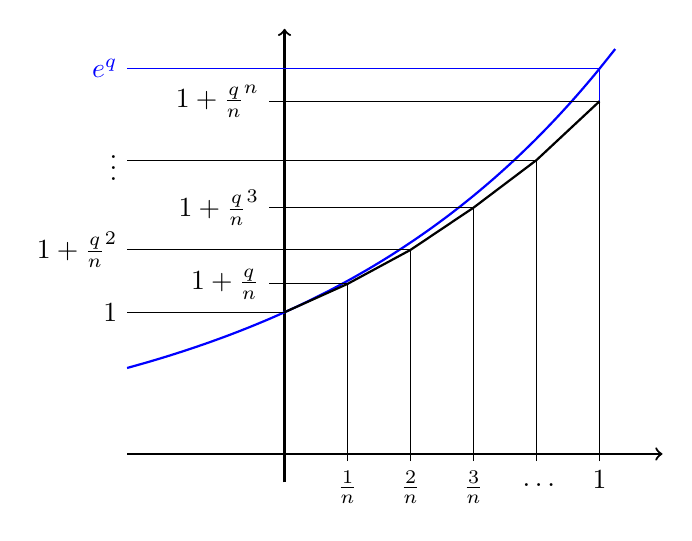
\begin{tikzpicture}[x=4.0cm,y=1.8cm]
    	\draw[thick,->] (-0.5,0) -- (1.2,0);
      \draw[thick,->] (0,-0.2) -- (0,3.0);
      %
      \draw[domain=-0.5:1.05,smooth,variable=\x,thick,blue] plot
      ({\x}, {exp(\x)});
      \draw[blue] (1.0,-0.05) -- (1.0,{exp(1.0)})
      -- (-0.5, {exp(1.0)}) node[left]{$e^q$};
      \draw (-0.5,1) node[left]{$1$} -- (0,1);
      \draw (0.2,-0.05) node[below]{$\frac 1 n$} -- (0.2,1.2)
      -- (-0.05,1.2) node[left]{$1+\scriptsize \frac q n$};
      \draw (0.4,-0.05) node[below]{$\frac 2 n$} -- (0.4,1.44)
      -- (-0.5,1.44) node[left]{$\enclose{1+\scriptsize\frac q n}^2$};
      \draw (0.6,-0.05) node[below]{$\frac 3 n$} -- (0.6,1.738)
      -- (-0.05,1.738) node[left]{$\enclose{1+\scriptsize\frac q n}^3$};
      \draw (0.8,-0.05) node[below]{$\rule{0mm}{2mm}\dots$} -- (0.8,2.0736)
      -- (-0.5,2.0736) node[left]{$\vdots$};
      \draw (1.0,-0.05) node [below] {$1$} -- (1.0,2.48832)
      -- (-0.05,2.48832) node[left]{$\enclose{1+\scriptsize\frac q n}^n$};
      \draw[thick] (0,1) -- (0.2,1.2)
      -- (0.4,1.44) -- (0.6,1.738)
      -- (0.8,2.0736) -- (1.0,2.48832);
    \end{tikzpicture}
  \end{center}
  \caption{L'interesse composto.
  Se dividiamo l'intervallo $[0,1]$
  in $n$ parti (in figura $n=5$), al passo zero
  partiamo con un capitale pari ad $1$ e ad ogni
  passo di ampiezza $\frac 1 n$ moltiplichiamo
  il nostro capitale per $1+\frac q n$ (supponendo
  di avere un interesse pari a $q$ che
  nel tempo $\frac 1 n$ ci paga quindi $\frac q n$
  volte il nostro capitale).
  Dopo
  $n$ passi, cioè al tempo $1$, avremo
  un capitale pari a $\enclose{1+\frac q n}^n$.
  Se $n\to+\infty$ questa quantità tende ad $e^q$.}
  \label{fig:nepero}
\end{figure}


La funzione esponenziale è legata ad un modello di crescita che si trova spesso
in natura: la \myemph{crescita esponenziale}.
Prendiamo come esempio una popolazione di batteri che cresce senza
limitazioni di spazio e di nutrimento oppure
alla crescita di un capitale dovuto ad una rendita finanziaria.

Supponiamo che una popolazione che al tempo $t_0=0$
ammonta ad un certo numero $c$ di batteri, al tempo
$t>0$ raggiunga una numerosità $q(t,c)$.
Se lascio crescere la popolazione per un ulteriore
tempo $s>0$ troverò al tempo $t+s$ la stessa
popolazione che avrei al tempo $s$ se al tempo
zero fossi partito con la popolazione $q(t)$:
\[
  q(t+s,c) = q(s,q(t,c)).
\]
L'equazione precedente si chiama proprietà
di \emph{semigruppo}
\index{semigruppo}%
continuo.
Ma fissato $t$ la popolazione $q(t,c)$ deve
essere proporzionale a $c$ perché ogni batterio
ha la sua discendenza indipendentemente dalla numerosità
totale della popolazione. In pratica
si deve avere $q(t,c) = k(t) \cdot c$ per una opportuna
funzione $k(t)$ che non dipende da $c$.
Dunque
\[
  q(t+s,c)
  = q(s,q(t,c))
  = k(s) \cdot q(t,c)
  = k(s) \cdot k(t) \cdot c
\]
da cui
\[
  k(t+s) = k(s) \cdot k(t).
\]
In base al teorema~\ref{th:esponenziale}
possiamo affermare
che $k(t)$ è una funzione esponenziale $k(t)=a^t$
per una qualche costante $a$.
La costante $a$ può essere determinata mediante la formula:
\[
  a = k(1) = \frac{q(1,c)}{c}
\]
ma questa espressione non ha un preciso significato fisico in quanto
dipende dall'unità di tempo scelta.

La costante a cui possiamo dare significato è invece l'aumento relativo
istantaneo della popolazione. Possiamo infatti supporre che
se lasciamo la popolazione crescere per un tempo $\Delta t$ molto piccolo,
si otterrà un aumento di popolazione proporzionale al tempo $\Delta t$
(stiamo qui anticipando il concetto di derivata) e alla popolazione:
\begin{equation}\label{eq:488464}
  q(\Delta t,c) = c + r c \Delta t = (1+r \Delta t) c.
\end{equation}
La costante $r$ rappresenta quindi l'aumento
relativo istantaneo della popolazione (nel caso dell'investimento
$r$ sarebbe il tasso di interesse istantaneo).
Questa definizione ha senso
quando $\Delta t$ è piccolo in quanto non tiene conto del fatto che
nell'intervallo di tempo $[t,t+\Delta t]$ la popolazione che si
è aggiunta genera anch'essa nuova popolazione (ovvero l'interesse
accumulato genera anch'esso interesse\footnote{%
In effetti la scoperta della costante $e$
è dovuta a Jacob Bernoulli nel 1683.
Bernoulli si chiedeva qual è l'interesse annuo effettivo
che si ottiene da un capitale che dia una rendita
giornaliera (interesse composto).
Se un capitale è investito ad un tasso di interesse $r$,
si intende che ogni giorno il capitale
viene aumentato di un fattore $1+r/365$
e quindi dopo un anno il fattore moltiplicativo è $(1+r/365)^365$.
}).

Per calcolare l'aumento della popolazione su tempi ``grandi'' possiamo
suddividere gli intervalli temporali in $n$ intervallini di ampiezza
$\Delta t$ e applicare in ognuno di essi la relazione \eqref{eq:488464}.
Si trova:
\begin{align*}
 q(\Delta t,c) &= c(1+r\Delta t) \\
 q(2\Delta t,c) &= q(\Delta t,c) (1+r\Delta t)  = c(1+r\Delta t)^2\\
 &\vdots \\
 q(n\Delta t) &= c(1+r\Delta t)^n.
\end{align*}
Dunque, ponendo $\Delta t=t/n$ si ha
\[
  q(t,c) = c\enclose{1+r\frac{t}{n}}^n
\]
in particolare per $t=1/r$ si ottiene:
\[
  q(1/r,c) = c\enclose{1+\frac{1}{n}}^n
\]
e ricordando che $q(t,c)=c a^t$ otteniamo:
\[
  a^{\frac 1 r} = \enclose{1+\frac{1}{n}}^n.
\]
Se per $n\to +\infty$ (che corrisponde a $\Delta t \to 0$)
la quantità sul lato destro tende ad un numero $e$ (che chiameremo costante
di Nepero) avremo allora
\[
  a = e^r, \qquad q(t,c) = c e^{rt}
\]
che è la relazione che lega le due costanti $a$ e $r$ che definiscono
la crescita esponenziale.

Risulta in effetti valido il seguente.

\begin{theorem}[costante di Nepero]
\mymark{**}
La successione
\[
  a_n = \enclose{1+\frac 1 n}^n
\]
è crescente e limitata, dunque è convergente.
\end{theorem}
%
\begin{proof}
Dimostriamo innanzitutto che $a_n$ è crescente, cioè che
per ogni $n\ge 2$ si ha $a_n \ge a_{n-1}$.
E' chiaro che $a_n>0$ per ogni $n$,
quindi ci riconduciamo a
verificare che $\frac{a_n}{a_{n-1}} \ge 1$.

Si ha
\begin{align*}
\frac{a_n}{a_{n-1}}
&= \frac{\enclose{1+\frac 1 n}^n}{\enclose{1+\frac 1 {n-1}}^{n-1}}
= \frac{\enclose{\frac{n+1}{n}}^n}{\enclose{\frac{n}{n-1}}^{n-1}}\\
&= \enclose{\frac{n+1}{n}\cdot\frac{n-1}{n}}^n \cdot \frac{n}{n-1}
= \enclose{\frac{n^2- 1}{n^2}}^n \cdot \frac{n}{n-1}
\end{align*}
Osserviamo ora che la disuguaglianza di Bernoulli garantisce
\[
  \enclose{\frac{n^2 -1}{n^2}}^n
  = \enclose{1-\frac{1}{n^2}}^n
  \ge 1 - \frac{n}{n^2} = 1 - \frac{1}{n} = \frac{n-1}{n}
\]
da cui si ottiene, come volevamo, $a_n / a_{n-1} \ge 1$ cioè
$a_n$ è crescente.

Se ora consideriamo la successione
\[
  b_n = \enclose{1+\frac 1 n}^{n+1}
\]
osserviamo che si ha
\[
  b_n = \enclose{1+\frac 1 n}^n \cdot \enclose{1+\frac 1 n}
   = a_n\cdot \enclose{1+\frac 1 n} > a_n.
\]
Per dimostrare che $a_n$ è limitata sarà quindi sufficiente dimostrare
che $b_n$ è superiormente limitata. Vedremo ora che $b_n$ è decrescente (e quindi $a_n \le b_n \le b_1$ è superiormente limitata).

Procediamo in maniera analoga a quanto fatto per $a_n$:
\begin{align*}
\frac{b_{n-1}}{b_n}
& = \frac{\enclose{1+\frac{1}{n-1}}^n}{\enclose{1+\frac{1}{n}}^{n+1}}
  = \frac{\enclose{\frac{n}{n-1}}^n}{\enclose{\frac{n+1}{n}}^{n+1}}
  = \enclose{\frac{n}{n-1}\cdot\frac{n}{n+1}}^{n+1}\cdot\frac{n-1}{n} \\
& = \enclose{\frac{n^2}{n^2-1}}^{n+1} \cdot \frac{n-1}{n}
  = \enclose{1 + \frac{1}{n^2-1}}^{n+1} \cdot \frac{n-1}{n}.
\end{align*}
In base alla disuguaglianza di Bernoulli otteniamo
\[
  \enclose{1 + \frac{1}{n^2-1}}^{n+1}
  \ge 1 + (n+1) \cdot \frac{1}{n^2-1}
  \ge 1 + \frac{1}{n-1} = \frac{n}{n-1}.
\]
Mettendo insieme le due stime si ottiene dunque $b_{n-1}/b_n \ge 1$
che è quanto ci rimaneva da dimostrare.
\end{proof}

E' quindi giustificata la seguente.

\begin{definition}[costante di Nepero]
\mymark{***}
Definiamo la \emph{costante di Nepero}%
\mynote{costante di Nepero}%
\index{costante!di Nepero}%
\index{$e$}%
\footnote{Nepero è l'italianizzazione del nome del
matematico scozzese John Napier (1550-1617).
Il nome $e$ è stato introdotto da Eulero (Leonhard Euler 1707-1783)
%http://eulerarchive.maa.org//docs/originals/E853.pdf
}
\[
  e = \lim_{n\to +\infty} \enclose{1+\frac 1 n}^n.
\]
\end{definition}

Sapendo che
\[
  \enclose{1+\frac 1 n}^n \le e \le \enclose{1+\frac 1 n}^{n+1}
\]
e ponendo $n=1$ otteniamo $2\le e \le 4$.

\begin{exercise}\label{ex:4876765}
Posto $a_n = \frac{n^n}{n!}$ mostrare che $\frac{a_{n+1}}{a_n} \to e$.
\end{exercise}

\begin{theorem}[limiti che si riconducono al numero $e$]
\mymargin{limiti che si riconducono al numero $e$}
Se $a_k \to 0$, $a_k\neq 0$ allora, per $k\to +\infty$,
\[
  \enclose{1+a_k}^{\frac 1 {a_k}} \to e.
\]
\end{theorem}
%
\begin{proof}
Caso 1. Se $a_k > 0$ allora consideriamo la successione di naturali
$n_k = \lfloor 1/a_k \rfloor$ cosicché
\[
  n_k \le \frac{1}{a_k} \le n_k + 1
\qquad
\text{e}
\qquad
 \frac{1}{n_k+1} \le a_k \le \frac 1 {n_k}.
\]
dunque
\[
\enclose{1+\frac 1 {n_k+1} }^{n_k}
  \le \enclose{1+a_k}^{\frac 1 {a_k}}
  \le \enclose{1+\frac 1 {n_k}}^{n_k + 1}.
\]
Osserviamo ora che essendo che per $k\to +\infty$ anche
$n_k \to +\infty$ si deve
avere (in base al teorema di cambio di variabile nei limiti)
\[
 \lim_k \enclose{1 + \frac{1} {n_k}}^{n_k+1}\!\!\!
 = \lim_n \enclose{1+ \frac 1 n}^{n+1}\!\!\!
 = \lim_n \enclose{1+ \frac 1 n}^n\!\cdot\enclose{1+\frac 1 n}
 = e
\]
ed essendo anche $n_k + 1 \to +\infty$
\[
  \lim_k \enclose{1 + \frac 1 {n_k+1}}^{n_k}
  = \lim_n \enclose{1+\frac 1 n}^{n-1}
  = \lim_n \frac{\enclose{1+\frac 1 n}^{n}}{1+\frac 1 n}
  = e.
\]
Dunque, per confronto tra i limiti, si ottiene $(1+a_k)^{\frac 1 {a_k}}\to e$.

Caso 2. Se $a_k<0$ possiamo scrivere $a_k = -\abs{a_k}$ da cui
\[
  \enclose{1+a_k}^{\frac 1 {a_k}}
  = \frac{1}{\enclose{1-a_k}^{\frac 1{a_k}}}
\]
e, procedendo come nel caso precedente, ci si riconduce al limite
\[
  \lim_n \frac{1}{\enclose{1-\frac 1 n}^n}.
\]
Per quest'ultimo osserviamo che si ha
\[
 \frac{1}{\enclose{1-\frac 1 n}^n}
 = \frac{1}{\enclose{\frac{n-1}{n}}^n}
 = \enclose{\frac{n}{n-1}}^n
 = \enclose{1 + \frac{1}{n-1}}^n
\]
che per quanto visto in precedenza (mettendo $n+1$ al posto di $n$)
ha anch'esso limite $e$.

Caso generale. Se $a_k$ ha segno variabile posso considerare
le due sottosuccessione dei termini di segno positivo e dei termini di segno
negativo. Per quanto visto nei casi precedenti entrambe le successioni
convergono ad $e$ e quindi è immediato verificare che l'intera
successione converge ad $e$.
\end{proof}

\begin{corollary}%
\label{cor:limite_notevole_ex}%
\mymark{**}%
Per ogni $x\in \RR$ si ha
\[
  \lim_{n\to +\infty} \enclose{1+ \frac x n}^n = e^x.
\]
\end{corollary}
%
\begin{proof}
Infatti, per il teorema precedente, posto $a_n = x/n$ si ha
\[
\lim_{n\to +\infty}\enclose{1+\frac x n}^{\frac n x} = e.
\]
Ma allora
\[
\enclose{1+ \frac x n}^n = \enclose{\enclose{1+\frac x n}^{\frac n x}}^x
\to e^x
\]
\end{proof}

\begin{definition}[logaritmi naturali]
Vedremo che il numero $e$ risulta essere una base naturale per la funzione
esponenziale e di conseguenza per il logaritmo. Il logaritmo in base
$e$ viene chiamato \myemph{logaritmo naturale} e viene indicato con $\ln = \log_e$.
\end{definition}

In alcuni testi si utilizza l'operatore $\log$, indicato senza una base esplicita,
ma la definizione non è completamente condivisa.
In certi testi (per lo più in ambito matematico)
si definisce $\log  = \ln = \log_e$,
in altri testi si considera $\log = \log_{10}$.

\begin{corollary}[limiti notevoli]\label{cor:limite_notevole_e}
\mymark{*}%
Se $a_n \to 0$, $a_n>0$ allora
\begin{gather}
 \lim_{n\to +\infty} \frac{\ln \enclose{1+ a_n}}{a_n} = 1; \\
 \lim_{n\to +\infty} \frac{e^{a_n}-1}{a_n} = 1.
\end{gather}
\end{corollary}
%
\begin{proof}
Per quanto riguarda il logaritmo ci si riconduce al teorema precedente
osservando che:
\[
  \frac{\ln(1+a_n)}{a_n}
  = \ln \enclose{(1+a_n)^{\frac 1 {a_n}}}.
\]
Per quanto riguarda l'esponenziale ci si riconduce al logaritmo
osservando che posto
\[
  b_n = e^{a_n}-1
\]
se $a_n\to 0$ anche $b_n\to 0$ e quindi si ha:
\[
\frac{e^{a_n}-1}{a_n} = \frac{b_n}{\ln(1+b_n)} \to 1.
\]

\end{proof}

\begin{exercise}
Mostrare che
\begin{gather*}
  \lim_{n\to+\infty} n^n\cdot \enclose{\frac{n+1}{n^2+1}}^n = e; \\
  \lim_{n\to+\infty} n\cdot \ln\enclose{1 + \frac 1 n} = 1; \\
  \lim_{n\to+\infty} \enclose{1-\frac{n+1}{n!}}^{(n-1)!} = \frac 1 e; \\
  \lim_{n\to+\infty} n \cdot \enclose{\sqrt[n]{2}-1} = \ln 2.
\end{gather*}
\end{exercise}

%%%%%%%%%%%%%%%%%%%
%%%%%%%%%%%%%%%%%%%
%%%%%%%%%%%%%%%%%%%
%%%%%%%%%%%%%%%%%%%
\section{criteri del rapporto e della radice}

Succede spesso di dover determinare il limite
del rapporto di due successioni che tendono entrambe a infinito
oppure entrambe a zero.
In queste situazioni il teorema del limite del rapporto non
si applica in quanto siamo di fronte ad una forma indeterminata.
Dovremo quindi capire quale delle due successioni
tende a infinito o a zero ``più velocemente''.

I teoremi che seguono si basano (in maniera più o meno implicita)
sull'andamento della successione geometrica:
\[
  a_n = q^n
\]
dove $q>0$ è una costante fissata.
Grazie al teorema~\ref{th:limite_esponenziale}
sappiamo che se $q>1$ si ha $q^n\to \infty$.
Se $q=1$ chiaramente $q^n=1\to 1$
e se $q<1$ si ha $q^{-1}>1$ e quindi $q^{-n} \to +\infty$
da cui $q^n \to 0$.

\begin{theorem}[criterio del rapporto]
\label{th:criterio_rapporto}
\index{criterio!del rapporto per le successioni}
\index{rapporto!criterio del}
  Sia $a_n$ una successione reale a termini non negativi
  $a_n \ge 0$ tale che esista il limite del rapporto di due termini consecutivi:
  \[
     \frac{a_{n+1}}{a_n} \to \ell \in [0,+\infty].
  \]
  Se $\ell < 1$ allora $a_n \to 0$, se $\ell >1$ allora $a_n \to +\infty$.
\end{theorem}
%
\begin{comment}
\begin{proof}\footnote{%
  la dimostrazione di questo teorema si potrebbe fare in maniera
  molto simile alla dimostrazione del teorema~\ref{th:criterio_radice}
  senza tirare in ballo il teorema~\ref{th:criterio_cesaro} che è decisamente più complesso.
  }
Grazie al teorema~\ref{th:criterio_cesaro} sappiamo
che $\sqrt[n]{a_n}\to \ell$ e quindi il risultato
segue direttametne dal teorema~\ref{th:criterio_radice}.
\end{proof}
\end{comment}

\begin{proof}
Supponiamo sia $\ell<1$. Posto $q=(1+\ell)/2$ si ha $\ell < q < 1$ e posto $\eps=q-\ell>0$ per la definizione di limite $\frac{a_{n+1}}{a_n}\to \ell$ dovrà esistere un $N\in \NN$ tale
che per ogni $n\ge N$ si abbia:
\[
  \frac{a_{n+1}}{a_n} < \ell + \eps = q
\]
ovvero $a_{n+1} < q \cdot a_n$. In particolare si avrà:
\begin{align*}
  a_{N+1} &< q \cdot a_N \\
  a_{N+2} &< q \cdot a_{N+1} < q^2\cdot a_N \\
  a_{N+3} &< q \cdot a_{N+2} < q^3\cdot a_N \\
  \vdots
\end{align*}
ed è chiaro che per induzione potremo dimostrare che per
ogni $k\in \NN$ si ha
\[
  a_{N+k} < q^k\cdot a_N.
\]
Osserviamo però che $q^k \cdot a_N \to 0$ per $k\to +\infty$
in quanto $q<1$ e quindi $q^k \to 0$. Dunque, tolti i primi $N$ termini, la successione $a_n$ tende a zero. Ma i primi $N$ termini non influenzano né il carattere né il limite della successione e quindi l'intera successione $a_n$ tende a zero.

Il caso $\ell>1$ si fa in maniera analoga. Si sceglie $q$ tale
che $1<q<\ell$ e si trova, in maniera analoga al caso precedente,
che per un certo $N\in \NN$ e per ogni $k\in \NN$ si ha
\[
  a_{N+k} > q^k \cdot a_N \to +\infty.
\]
\end{proof}

Osserviamo che, nel teorema precedente (ma anche nel criterio della radice teorema~\ref{th:criterio_radice}),
non si può concludere alcunché nel
caso in cui sia $\ell = 1$.
Ad esempio le due successioni $a_n = 1/n$ e $b_n = n$
hanno limiti diversi ($a_n \to 0$, $b_n\to +\infty$) ma per entrambe
il limite del rapporto di termini consecutivi tende ad $\ell=1$.

\begin{exercise}
Mostrare che
\begin{gather*}
  \lim \frac{n!}{n^n} = 0 \\
  \lim \frac{(2n)!}{(2n)^n} = +\infty
\end{gather*}
\end{exercise}

\begin{theorem}[criterio della radice]
\label{th:criterio_radice}%
\mymark{***}%
\mynote{criterio della radice}%
\index{criterio!della radice per successioni}%
Sia $a_n$ una successione a termini positivi tale che
\[
  \sqrt[n]{a_n} \to \ell
\]
con $\ell \in \bar \RR$.
Allora se $\ell<1$ si ha $a_n \to 0$ se invece $\ell > 1$ si ha $a_n \to +\infty$.
\end{theorem}
%
\begin{comment}
\begin{proof}
\mymark{**}
Consideriamo prima il caso $\ell < 1$.
Se $\lim \sqrt[n]{a_n} = \ell$ significa che per ogni $\eps>0$ la successione
$\sqrt[n]{a_n}$ risulta definitivamente minore di $\ell +\eps$.
Scegliendo opportunamente $\eps$ (ad esempio $\eps = (1-\ell)/2$) si potrà
avere $q = \ell+\eps < 1$. Dunque avremo definitivamente $\sqrt[n]{a_n}< q$
ovvero $a_n < q^n$. Per ipotesi $a_n\ge 0$
e quindi, tolto un numero finito di termini, si ottiene $0 \le a_n < q^n \to 0$
da cui $a_n \to 0$ (in quanto l'aver tolto un numero finito di termini non
cambia né il carattere né il limite della successione).

Se $\ell>1$ si potrà procedere in maniera analoga. Esisterà $q$ con $1 < q < \ell$ tale che definitivamente $\sqrt[n]{a_n} > q$ da cui $a_n > q^n \to +\infty$.
\end{proof}
\end{comment}

\begin{proof}
  Si può osservare che
  \[
    a_n = \enclose{\sqrt[n]{a_n}}^n
     = e^{n \cdot \ln \sqrt[n]{a_n}}.
  \]
  Se $\ell <1$ allora il logaritmo tende ad un numero negativo,
  l'argomento dell'esponenziale tende a $-\infty$ e quindi l'esponenziale tende a zero (teorema~\ref{th:limite_esponenziale}).

  Se invece $\ell>1$ il logaritmo tende ad un numero positivo e quindi l'esponenziale tende a $+\infty$.
\end{proof}

\begin{theorem}[convergenza alla Cesàro]
\label{th:criterio_cesaro}%
\mymark{*}%
\mymargin{Cesàro}%
\index{criterio!del rapporto alla Cesàro}%
\index{somma!di Cesàro}%
Sia $a_n$ una successione a termini positivi.
\begin{enumerate}
\item
  Se
  $   a_n \to \ell \in \bar \RR$
  allora
  \[
  \frac{a_1 + \dots + a_n}{n} \to \ell.
  \]

\item
  Se $a_n>0$,
  $\displaystyle\frac{a_{n+1}}{a_n} \to \ell \in [0,+\infty]$
  allora
  $\displaystyle \sqrt[n]{a_n}\to \ell$.
\end{enumerate}
\end{theorem}
%
\begin{proof}
Dimostriamo il primo punto.
Se $\ell\in \RR$ possiamo scrivere
\begin{align*}
b_n &= \abs{\frac{a_1 + \dots + a_n}{n} - \ell}
  = \abs{\frac{(a_1-\ell) + \dots + (a_n-\ell)}{n}}\\
  &\le \frac{\abs{a_1-\ell} + \dots + \abs{a_n-\ell}}{n}.
\end{align*}
Sapendo che $a_n\to \ell$ per ogni $\eps>0$
esiste $N\in \NN$ tale che per ogni $n>N$ si ha
$\abs{a_n-\ell}<\eps$.
Dunque continuando le disuguaglianze precedenti,
se $n>N$
si ha
\[
b_n \le \frac{\abs{a_1-\ell} + \dots + \abs{a_N-\ell}}{n}
    + \frac{(n-N)\cdot\eps}{n}.
\]
Fissati $\eps$ e $N$ possiamo
passare al $\limsup$ per $n\to +\infty$
\[
\limsup_{n\to+\infty} b_n
\le 0 + \eps.
\]
Ma ovviamente il $\liminf b_n \ge 0$ e
dunque abbiamo mostrato che per ogni $\eps >0$ si ha
\[
0 \le \liminf_{n\to+\infty} b_n \le \limsup_{n\to+\infty} b_n \le \eps.
\]
Significa che $\limsup b_n = \liminf b_n = \lim b_n = 0$.

Se $a_n\to \ell=+\infty$ si ragiona in maniera simile.
Per ogni $M\in \RR$ esiste $N$ tale che per $n>N$ si ha $a_n>M$.
Dunque:
\[
  \frac{a_1+\dots + a_n}{n}
  \ge \frac{a_1 + \dots + a_N}{n} + \frac{(n-N)M}{n}
\]
e passando al $\liminf $ per $n\to +\infty$ si trova
\[
 \liminf_{n\to+\infty} \frac{a_1 + \dots + a_n}{n}
 \ge M
\]
che ci porta al risultato desiderato.
In maniera del tutto analoga si dimostra il caso $\ell=-\infty$.

Il punto 2 si può ricondurre all'1.
Infatti
\[
  \ln \sqrt[n]{a_n}
  = \ln \sqrt[n]{a_0\cdot \frac{a_1}{a_0} \cdots \frac{a_n}{a_{n-1}}}
  = \frac{\ln a_0 + \ln \frac{a_1}{a_0} + \dots + \ln \frac{a_n}{a_{n-1}}}{n}.
\]
Posto $x_n = \ln \frac{a_n}{a_{n-1}}$
se $\frac{a_n}{a_{n-1}}\to \ell$
si ha $x_n\to \ln \ell$ (intendendo $\ln 0 = -\infty$ e $\ln (+\infty)=+\infty$) e dunque
\[
  \ln \sqrt[n]{a_n} = \frac{\ln a_0}{n} + \frac{x_1 + \dots + x_n}{n}
  \to \ln \ell.
\]
Facendo l'esponenziale di ambo i membri si trova il risultato desiderato.
\end{proof}

\begin{exercise}
Si applichi il risultato precedente per
verificare che
\[
   \lim \sqrt[n]{n} = 1
\]
e
\[
  \lim \frac{n}{\sqrt[n]{n!}} = e.
\]
\end{exercise}

\begin{exercise}
Si consideri la successione
\[
a_n =
\begin{cases}
   2^n &\text{se $n$ pari},\\
   n\cdot 2^n &\text{se $n$ dispari}.
\end{cases}
\]
Verificare che alla successione $a_n$
si può applicare il criterio della radice ma
non il criterio del rapporto.
Usare questo esempio per mostrare che le implicazioni
enunciate nel teorema~\ref{th:criterio_cesaro} non
possono essere invertite.
\end{exercise}

%%%%%
%%%%%
\section{ordini di infinito, equivalenza asintotica}
%%%%%
%%%%%

\begin{definition}[ordine di infinito/infinitesimo]
\label{def:ordine_infinito}
\mymark{***}%
\mymargin{ordine di infinito/infinitesimo}%
\index{ordine!di infinito}%
\index{infinito}%
\index{infinitesimo}%
Siano $a_n$ e $b_n$ successioni a termini positivi.
\begin{enumerate}
\item
Diremo che
per $n\to +\infty$ la successione $a_n$ è \emph{molto più piccola}
della successione $b_n$ e scriveremo $a_n \ll b_n$ se vale
\mymargin{$\ll$}
\[
\frac{a_n}{b_n} \to 0
\]
diremo invece che $a_n$ è \emph{molto più grande}
di $b_n$ e scriveremo $a_n \gg b_n$ se
\mymargin{$\gg$}
\[
\frac{a_n}{b_n} \to +\infty.
\]
\item
Diremo invece che $a_n$ e $b_n$
sono \myemph[equivalenza asintotica]{asintoticamente equivalenti}
\mymargin{equivalenza!asintotica}%
per $n\to+\infty$
e scriveremo $a_n \sim b_n$ se
\[
\mymargin{$\sim$}
\frac{a_n}{b_n} \to 1.
\]
\end{enumerate}
\end{definition}

Ad esempio è facile verificare che se $\alpha > \beta > 0$
allora $n^\alpha \gg n^\beta$ per $n\to +\infty$
e se $a>b>1$ allora $a^n\gg b^n$ per $n\to +\infty$.

E' molto facile verificare che le relazioni
$\ll$ e $\gg$ sono una l'inversa dell'altra
e soddisfano la proprietà transitiva
mentre la relazione $\sim$ soddisfa la proprietà simmetrica
e la proprietà transitiva.

\begin{theorem}[ordini di infinito]
\label{th:ordine_infinito}%
\mymargin{ordini di infinito}%
\mymark{***}%
Per ogni $a>1$, $\alpha>0$ si ha, per $n\to +\infty$
\[
\log_a n \ll n^\alpha \ll a^n \ll n! \ll n^n.
\]
Più in generale se $x_n \to +\infty$
è una qualunque successione si ha,
per $n\to+\infty$
\[
\log_a(x_n) \ll (x_n)^\alpha \ll a^{x_n}.
\]
\end{theorem}
%
\begin{proof}
\mymark{**}
Cominciamo col mostrare che $a^n \ll n!$
applicando il criterio del rapporto alla successione $\frac{a^n}{n!}$:
\[
\frac{\displaystyle \frac{a^{n+1}}{(n+1)!}}{\displaystyle \frac{a^n}{n!}}
= \frac{a^{n+1}}{a^n}\cdot \frac{n!}{(n+1)!}
= a \cdot \frac {1}{n + 1} \to 0 < 1.
\]
Dunque si ha, come richiesto $a^n / n! \to 0$.
Si procede in modo analogo per mostrare che $n! \ll n^n$:
\begin{align*}
\frac{(n+1)!}{n!}\cdot \frac{n^n}{(n+1)^{n+1}}
&= (n+1) \cdot \enclose{\frac{n}{n+1}}^n \frac {1}{n+1}\\
&= \frac{1}{\enclose{1+\frac 1 n}^n} \to \frac 1 e < 1.
\end{align*}

Per dimostrare che
$n^\alpha \ll a^n$
si può procedere con il criterio del rapporto, come nei casi precedenti:
\[
\frac{(n+1)^\alpha}{n^\alpha}\cdot \frac{a^n}{a^{n+1}}
= \frac 1 a \cdot \enclose{\frac{n+1}{n}}^\alpha \to \frac 1 a \cdot 1^\alpha = \frac 1 a < 1
\]
da cui $n^\alpha / a^n \to 0$.

Se ora $x_n\to +\infty$ è qualunque
cerchiamo di ricondurci ad una successione a valori interi.
Osserviamo che si ha
\[
\lfloor x_n \rfloor
\le x_n
\le \lfloor x_n \rfloor + 1
\]
da cui, per monotonia,
\[
\lfloor x_n \rfloor^\alpha
\le x_n^\alpha
\le (\lfloor x_n \rfloor + 1)^\alpha
= \lfloor x_n \rfloor^\alpha \enclose{1+ \frac{1}{\lfloor x_n \rfloor}}^\alpha
\]
e
\[
a^{\lfloor x_n \rfloor}
\le a^{x_n}
\le a^{\lfloor x_n \rfloor + 1}
= a \cdot a^{\lfloor x_n \rfloor}.
\]
Dunque
\[
\frac{\lfloor x_n \rfloor^\alpha}{a \cdot a^{\lfloor x_n \rfloor}}
\le \frac{x_n^\alpha}{a^{x_n}}
\le \frac{\lfloor x_n \rfloor^\alpha \enclose{1+ \frac{1}{\lfloor x_n \rfloor}}^\alpha}
    {a^{\lfloor x_n \rfloor}}.
\]
Ma ora, se $n\to +\infty$ sapendo che $\lfloor x_n\rfloor \to +\infty$ si ha
che (per il teorema di sostituzione del limite)
\[
\lim \frac{\lfloor x_n \rfloor^\alpha}{a^{\lfloor x_n \rfloor}} = 0
\qquad
\text{e}
\qquad
\lim \frac{\lfloor x_n \rfloor^\alpha }
    {a^{\lfloor x_n \rfloor}} = 0
\]
da cui segue che $\frac{x_n^\alpha}{a^{x_n}}\to 0$.

Per dimostrare l'ultima relazione, $\log_a(x_n)\ll (x_n)^\alpha$,
consideriamo la successione $y_n = \alpha \cdot \log_a x_n$
cosicché $a^{y_n} = x_n^\alpha$.
Notiamo che se $x_n\to +\infty$
anche $y_n \to +\infty$.
Dunque, per le proprietà precedenti,
sappiamo che $y_n \ll a^{y_n}$ e dunque
\[
\frac{\log_a x_n}{x_n^\alpha}
= \frac{1}{\alpha}\cdot\frac{y_n}{a^{y_n}} \to 0.
\]
\end{proof}

Le notazioni e gli
ordini di infinito individuati nel teorema precedente
sono strumenti molto utili nel calcolo dei limiti.

L'equivalenza asintotica
si mantiene per prodotto e rapporto:
se $a_n\sim A_n$ e $b_n\sim B_n$ allora
\[
 a_n \cdot b_n \sim A_n \cdot B_n,
 \qquad
 \frac{a_n}{b_n} \sim \frac{A_n}{B_n}.
\]
Osserviamo inoltre che se
$a_n \sim b_n$ e se $a_n\to \ell$ allora
anche $b_n\to \ell$.
Se poi $\ell\in(0,+\infty)$
la relazione $a_n\sim \ell$ è equivalente ad $a_n\to \ell$.

Per quanto riguarda la somma
è facile verificare che se $a_n\ll b_n$ allora
$a_n+b_n \sim b_n$ in quanto
\[
  \frac{a_n + b_n}{b_n} = \frac{a_n}{b_n} + 1 \to 1.
\]

In un limite in cui compaiono somme di termini
di ordini diversi potremo allora raccogliere i termini di ordine
massimo per individuare il limite, come facciamo
nel seguente.

\begin{example}
Calcolare il limite
\[
\lim_{n\to+\infty}
\frac{2n^4 + 3^n - 3 \ln n}{n! - 3\sqrt n}.
\]
\end{example}
\begin{proof}[Svolgimento.]
Si ha
\[
\frac{2n^4 + 3^n - 3 \ln n}{n! - 3\sqrt{n}}
= \frac
{3^n \cdot \enclose{2\frac{n^4}{3^n}+ 1 - 3\frac{\ln n}{3^n}}}
{n!\cdot \enclose{1-3\frac{\sqrt n}{n!}}}
\]
e ricordando che risulta (teorema~\ref{th:ordine_infinito})
\[
n^4 \ll 3^n, \qquad
\ln n \ll 3^n, \qquad
\sqrt n \ll n!, \qquad
3^n \ll n!
\]
avremo
\[
\frac{2n^4 + 3^n - 3 \ln n}{n! - 3\sqrt{n}}
\sim \frac{3^n}{n!} \to 0.
\]
\end{proof}


\begin{exercise}
Calcolare i seguenti limiti
\begin{gather*}
  \lim_{n\to +\infty} \frac{\displaystyle \ln\sqrt{n^2+n^n}}
  {\displaystyle e^{1 + \ln n}\cdot \ln(n^2-n\sqrt n)}, \qquad
  \lim_{n\to +\infty} \frac{\sqrt{n! + 2^n}}{3^n}, \\
  \lim_{n\to +\infty} \frac{\sqrt{(2n)!}}{n^n}, \qquad
  \lim_{n\to +\infty} \sqrt[n]{e^n + \sqrt{10^n}}.
\end{gather*}
\end{exercise}

\section{il teorema degli zeri}

\begin{theorem}[degli zeri]
\mymark{***}%
\mynote{teorema degli zeri}%
\index{teorema!degli zeri}%
\label{th:zeri}%
Sia $I\subset \RR$ un intervallo, $f\colon I \to \RR$ una funzione
continua, $a,b\in I$ tali che $f(a)\le 0$ e $f(b)\ge 0$.
Allora esiste $c\in I$ tale che $f(c)=0$.
\end{theorem}

\begin{proof}
\mymark{***}
La dimostrazione che adottiamo è di particolare rilevanza in quanto
non solo permette di dimostrare l'esistenza del punto $c$ che risolve
$f(x)=0$
ma ci presenta
un algoritmo, il \myemph{metodo!di bisezione},
\index{bisezione!metodo di}
che può essere effettivamente utilizzato per approssimare
tale soluzione.

Possiamo supporre senza perdere di  generalità che sia $a<b$.
Poniamo $A_0 = a$, $B_0= b$ e consideriamo il punto medio $C_0 = (A_0+B_0)/2$.
Scegliamo tra i due intervalli $[A_0, C_0]$ e $[C_0,B_0]$ quello per cui
il segno ai due estremi è discorde (o, caso fortunato, nullo).
Più precisamente se $f(C_0)\ge 0$ poniamo $[A_1,B_1] = [A_0,C_0]$ altrimenti
scegliamo $[A_1,B_1] = [C_0,B_0]$ così si ha, in ogni caso,
$f(A_1)\le 0$, $f(B_1)\ge 0$.

Consideriamo il punto medio $C_1$ del nuovo intervallo $[A_1,B_1]$ e ripetiamo
il procedimento indefinitamente. Quello che otteniamo sono due successioni
$A_n$, $B_n$ con queste proprietà (che potrebbero essere dimostrate per induzione):
\begin{enumerate}
\item $A_n < B_n$, $B_n - A_n = (b-a)/2^n$;
\item $A_n$ è crescente, $B_n$ è decrescente;
\item $f(A_n)\le 0$, $f(B_n)\ge 0$.
\end{enumerate}

Essendo $A_n$ monotòna sappiamo che $A_n$ converge $A_n\to c$.
Inoltre visto che $A_n \in [a,b]$ anche $c\in [a,b]$ (per la permanenza del
segno delle successione $A_n-a$ e $b-A_n$).
Passando al limite nell'uguaglianza $B_n = A_n + (b-a)/2^n$
si ottiene che anche $B_n \to c$. Essendo $f$ continua
avremo
\[
f(A_n) \to f(c), \qquad
f(B_n) \to f(c).
\]
Ma $f(A_n)\le 0$ e quindi per la permanenza del segno anche $f(c)\le 0$.
D'altra parte $f(B_n) \ge 0$ e quindi $f(c)\ge 0$.
Si ottiene dunque $f(c) = 0$, come volevamo dimostrare.
\end{proof}

\begin{example}\label{ex:75445}
Si voglia risolvere l'equazione
\[
  x^5-x-1=0.
\]
Posto $f(x) = x^5-x-1$ è chiaro che la funzione $f\colon \RR\to \RR$
è continua (in quanto composizione di funzioni continue).
Osserviamo che $f(0) = -1$ e $f(2)=29$, dunque la funzione
soddisfa le ipotesi del teorema degli zeri sull'intervallo $[0,2]$.
Sappiamo quindi che l'equazione in questione ha almeno una soluzione
in tale intervallo.

Utilizzando il metodo di bisezione possiamo determinare una soluzione
con precisione arbitraria. Posto $A_0=0$, $B_0=2$ abbiamo verificato che
$f(A_0)<0$ e $f(B_0)>0$.
Prendiamo il punto
medio $C_0=1$ e calcoliamo la funzione: $f(C_0)=-1 < 0$. Sappiamo
allora che una soluzione deve essere compresa nell'intevallo
$[A_1,B_1] = [C_0,B_0] = [1,2]$ perché anche in tale intervallo valgono le ipotesi
del teorema degli zeri.
Il punto medio di tale intervallo è $C_1=3/2 = 1.5$
e risulta $f(3/2) = 163/32>0$ dunque l'intervallo successivo
che andremo a considerare è $[A_2,B_2]=[1,3/2]$.
Per non dover lavorare con troppe cifre decimali invece di suddividere
esattamente a metà quest'ultimo intervallo consideriamo un punto
intermedio $C_2 = 6/5 = 1.2$ dove si ha $f(C_2)=901/3125>0$.
Sappiamo allora che una soluzione è compresa nell'intervallo
$[A_3,B_3] = [1,1.2]$. Prendiamo il punto medio $C_3=11/10=1.1$
e troviamo $f(C_3) = -48949/10^5 <0$. Abbiamo quindi ottenuto
che esiste $x\in (1.1,1.2)$ tale che $f(x)=0$. Sappiamo quindi
che $\abs{x-1.15} < 0.05$ cioè abbiamo trovato $x$ con un errore
inferiore a $0.05$.

Con molta pazienza si può procedere
con il metodo di bisezione fino ad arrivare a verificare
che $f(116/10^2)$ $=$ $-596583424/10^{10}<0$ e $f(117/10^2)=224480357/10^{10}>0$ da cui
si ottiene che una soluzione è compresa tra $1.16$ e $1.17$ con un errore
inferiore a $0.005$.
Con il calcolatore (si veda ad esempio il codice a pagina \pageref{code:bisection})
si possono ottenere più cifre significative: $x=1.1673039782614187\ldots$
\end{example}

\begin{table}
\begin{center}
\begin{tabular}{r}
$\sqrt 2 \approx $ 1.\small
4142135623 7309504880 1688724209 6980785696 7187537694 \\ \small
8073176679 7379907324 7846210703 8850387534 3276415727 \\
% 3501384623 0912297024 9248360558 5073721264 4121497099 \\ \small
% 9358314132 2266592750 5592755799 9505011527 8206057147 \\ \small
% 0109559971 6059702745 3459686201 4728517418 6408891986 \\ \small
% 0955232923 0484308714 3214508397 6260362799 5251407989 \\ \small
% 6872533965 4633180882 9640620615 2583523950 5474575028 \\ \small
% 7759961729 8355752203 3753185701 1354374603 4084988471 \\ \small
% 6038689997 0699004815 0305440277 9031645424 7823068492 \\ \small
% 9369186215 8057846311 1596668713 0130156185 6898723723 \\ \small
% 5288509264 8612494977 1542183342 0428568606 0146824720 \\ \small
% 7714358548 7415565706 9677653720 2264854470 1585880162 \\ \small
% 0758474922 6572260020 8558446652 1458398893 9443709265 \\ \small
% 9180031138 8246468157 0826301005 9485870400 3186480342 \\ \small
% 1948972782 9064104507 2636881313 7398552561 1732204024 \\ \small
% 5091227700 2269411275 7362728049 5738108967 5040183698 \\ \small
% 6836845072 5799364729 0607629969 4138047565 4823728997 \\ \small
% 1803268024 7442062926 9124859052 1810044598 4215059112 \\ \small
% 0249441341 7285314781 0580360337 1077309182 8693147101 \\ \small
% 7111168391 6581726889 4197587165 8215212822 9518488472 \\
\\
$\sqrt 3 \approx$ 1.\small
7320508075 6887729352 7446341505 8723669428 0525381038 \\ \small
0628055806 9794519330 1690880003 7081146186 7572485757 \\
\\
$\phi = \frac{\sqrt 5+1}{2} \approx $ 1.\small
6180339887 4989484820 4586834365 6381177203 0917980576 \\ \small
2862135448 6227052604 6281890244 9707207204 1893911375
  \end{tabular}
\end{center}
\caption{Le prime 100 cifre decimali di alcune
costanti calcolate con il metodo di bisezione usato nella dimostrazione
del teorema~\ref{th:zeri}.
Si veda il codice a pagina~\pageref{code:bisection}.}
\label{fig:cifre_sqrt2}
\index{$\sqrt 2$!cifre decimali}
\index{cifre!$\sqrt 2$}
\end{table}

\begin{corollary}[proprietà dei valori intermedi]
\mymark{**}
\mymargin{proprietà!dei valori intermedi}
Sia $I\subset \RR$ un intervallo e $f\colon I \to \RR$ una
funzione continua.
Allora se $f$ assume due valori $y_1$ e $y_2$ allora $f$
assume anche tutti i valori intermedi tra $y_1$ e $y_2$.
Detto altrimenti: una funzione continua
manda intervalli in intervalli.
\end{corollary}
%
\begin{proof}
Se $y_1$ e $y_2$ sono valori assunti da $f$ significa
che esistono $x_1,x_2 \in I$ tali che $f(x_1)= y_1$ e $f(x_2)=y_2$.
Allora scelto $y$ si consideri la funzione $g(x) = f(x)-y$.
Se $y$ è intermedio tra $y_1$ e $y_2$ la funzione $g$ assumerà
segni opposti in $x_1$ e $x_2$ e dunque, per il teorema degli zeri,
dovrà esserci un punto $x$ in cui $g$ si annulla. In tale punto
si avrà dunque $f(x)=y$, come volevamo dimostrare.
\end{proof}

\begin{lemma}
Se $I$ è un intervallo di $\RR$ ogni funzione $f\colon I \to \RR$
iniettiva e continua è strettamente monotona.
\end{lemma}
%
\begin{proof}
Si può osservare che una funzione è strettamente monotona se mantiene i valori
intermedi cioè se dati tre punti
$x<y<z$ risulta sempre che $f(y)$ è un valore intermedio tra $f(x)$ e $f(z)$:
\[
  f(x)< f(y) <f(z) \qquad\text{oppure} \qquad f(x)> f(y) > f(z).
\]
Se ciò non accadesse, ad esempio se fosse $f(y)>f(z)>f(x)$ con $x<y<z$
allora per la continuità di $f$ dovrebbe esistere un valore intermedio
tra $x$ e $y$ in cui la funzione assume il valore $f(z)$. Ma allora la funzione
non sarebbe iniettiva.
\end{proof}

%%%%%%%%%%%%%%%%%%%%%%%%
%%%%%%%%%%%%%%%%%%%%%%%%
%%%%%%%%%%%%%%%%%%%%%%%%
%%%%%%%%%%%%%%%%%%%%%%%%
\section{il teorema di Weierstrass}

Ricordiamo che nella definizione~\ref{def:funzione_limitata}
abbiamo definito i concetti di massimo, minimo, estremo superiore
e inferiore di una funzione a valori reali.

\begin{lemma}[successioni minimizzanti/massimizzanti]
\mynote{successioni mi\-ni\-miz\-zan\-ti/mas\-si\-miz\-zan\-ti}
\index{successioni!minimizzanti}
\index{successioni!massimizzanti}
Sia $A$ un insieme non vuoto e
sia $f\colon A \to \RR$ una funzione. Allora esistono
due successioni $a_n$ e $b_n$ di punti di $A$ tali che
\[
  \lim_{n\to +\infty} f(a_n) = \inf f(A), \qquad
  \lim_{n\to +\infty} f(b_n) = \sup f(A).
\]
\end{lemma}
%
\begin{proof}
Ricordiamo che $f(A) = \ENCLOSE{f(x)\colon x \in A}$ è l'immagine
della funzione $f$. Facciamo la dimostrazione per l'estremo inferiore,
risultato analogo si potrà ottenere per l'estremo superiore.

Sia $m=\inf f(A)$.
Se $m=-\infty$ significa che $f(A)$ non è inferiormente limitato,
in particolare per ogni $n\in \RR$ esiste $a_n$ tale che
$f(a_n) < - n$.
Dunque (per confronto) $f(a_n) \to -\infty$
come volevamo dimostrare.

Se $m\in \RR$ per le proprietà caratterizzanti l'estremo inferiore
sappiamo che per ogni $\eps>0$ esiste $a\in A$ tale che
$f(a) < m + \eps$.
Per ogni $n\in\NN$ possiamo scegliere $\eps=1/n$ e ottenere quindi
una successione $a_n$ tale che $f(a_n) < m + 1/n$.
D'altra parte essendo $m$ un minorante di $f(A)$ sappiamo che
$m \le f(a_n)$.
Abbiamo dunque $m \le f(a_n) < m+ 1/n$ e per il teorema dei
carabinieri possiamo quindi concludere che $f(a_n) \to m$
per $n\to +\infty$.
\end{proof}

\begin{theorem}[Weierstrass]%
\mymark{***}%
\mynote{teorema di Weierstrass}%
\index{teorema!di Weierstrass}%
\footnote{%
Probabilmente già dal IX secolo a.C.\ era noto ai greci che la circonferenza, tra tutte le figure piane che racchiudono una area prefissata, è quella di lunghezza minima. Dimostrare questa proprietà del cerchio (chiamata proprietà isoperimetrica) non è semplice ma può essere fatto con gli strumenti classici della geometria euclidea (si veda anche il problema di Didone, raccontato da Virgilio nella fondazione di Cartagine).
\index{isoperimetrico!problema}%
\index{problema!isoperimetrico}%
\index{problema!di Didone}%
L'analogo problema si può formulare nello spazio ovvero: tra tutte le regioni dello spazio di un certo volume prefissato determinare quella la cui frontiera ha superficie di area minima.
Anche in questo caso fin dai tempi antichi si è ipotizzato che la soluzione
di questo problema fosse la sfera, ma una dimostrazione è mancata fino agli inizi del 1800. Eulero (Leonhard Euler 1707--1783)
\index{Euler!Leonhard}%
\index{Eulero}%
pensò di aver
trovato una dimostrazione
che si fondava su questo risultato:
presa una qualunque superficie chiusa nello spazio,
se questa non è una sfera è possibile
farne una piccola modifica in modo da ottenere una nuova superficie
che racchiude lo stesso volume ma che ha area strettamente inferiore.
Fu proprio Karl Weiestrass (1815--1897)
\index{Weiestrass!Karl}%
ad accorgersi che quanto dimostrato da Eulero non è sufficiente a garantire la minimalità della sfera. Infatti Eulero
dimostra che non ci può essere un minimo che non sia la sfera, ma non dimostra che il minimo esiste e quindi non è detto che la sfera sia il minimo: potrebbero esserci infinite superfici $S_1, S_2, \dots, S_n, \dots$ ognuna con area minore di quella della sfera e ognuna con area maggiore della successiva: $A(S_{n+1})< A(S_n)$. Per concludere il ragionamento di Eulero era necessario dimostrare che in una situazione del genere le superifici $S_n$ debbano, in qualche senso, tendere alla superficie sferica e che le loro aree debbano
tendere all'area della sfera. In astratto questo è quanto viene enunciato nel teorema che porta il suo nome.
Dunque Weiestrass completò la dimostrazione della proprietà isoperimetrica
della sfera in dimensione $n=3$.
La dimostrazione dello stesso risultato in dimensione qualunque $n>3$ è invece
ancora più recente e si deve a Ennio De Giorgi (1928--1996)
\index{De Giorgi!Ennio}%
che formalizzò il concetto di perimetro introdotto
da Renato Caccioppoli (1904--1959).%
\index{Caccioppoli!Renato}%
\index{Caccioppoli!perimetro}%
}
Siano $a,b\in \RR$ con $a\le b$
e sia $f\colon [a,b]\to \RR$ una funzione continua.
Allora
esistono punti di massimo e di minimo per $f$ su $[a,b]$.
\end{theorem}
%
\begin{proof}
\mymark{***}
Dimostriamo solamente che $f$ ha minimo, per il massimo la dimostrazione procede
infatti in maniera del tutto analoga.

Sia $m= \inf f([a,b])$.
Per il lemma precedente sappiamo che esiste una successione $a_n$ minimizzante ovvero tale che
$a_n \in A$ e $f(a_n)\to m$ per $n\to +\infty$.

Per il teorema di Bolzano-Weierstrass dalla successione $a_n$ possiamo estrarre una sottosuccessione $a_{n_k}$ convergente: $a_{n_k} \to x_0$.
Visto che $a_{n_k} \in [a,b]$ si avrà, per il teorema della permanenza del segno, anche $x_0 \in [a,b]$ (si applichi la permanenza del segno alle successioni $a_{n_k}-a$ e $b-a_{n_k}$).

Dunque abbiamo una successione $a_{n_k}\to x_0$ con $a_{n_k}\in [a,b]$ e
$x_0 \in [a,b]$. Essendo $f$ continua si avrà dunque $f(a_{n_k}) \to f(x_0)$.
Ma noi sapevamo che $f(a_n)\to m$ e dunque anche $f(a_{n_k}) \to m$.
Concludiamo quindi che $f(x_0) = m$ cioè $m$, l'estremo inferiore,
è un valore assunto dalla funzione ed è quindi un minimo.
Dal canto suo $x_0$ è un punto di minimo assoluto.
\end{proof}

\begin{corollary}[limitatezza delle funzioni continue]
Sia $f\colon [a,b]\to \RR$ una funzione continua. Allora $f$ è limitata.
\end{corollary}
\begin{proof}
Visto che $f$ ha massimo $M$ e minimo $m$ si ha $f(x)\in [m,M]$ per ogni $x\in[a,b]$.
Ovviamente $m>-\infty$ e $M<+\infty$ in quanto $m$ e $M$ sono valori della funzione $f$.
\end{proof}

%%%%%%%%%%%%%%%%%
%%%%%%%%%%%%%%%%%
%%%%%%%%%%%%%%%%%
%%%%%%%%%%%%%%%%%

\section{successioni ricorsive}

Le successioni ricorsive sono le successioni
definite per induzione (tramite il teorema~\ref{th:induzione}):
\[
 \begin{cases}
   a_0 = \alpha \\
   a_{n+1} = f(a_n).
 \end{cases}
\]
Si rimanda al capitolo~\ref{ch:successioni_ricorsive}
per uno studio approfondito di questo tipo di successioni.
La prima parte di quel capitolo è infatti accessibile con le nozioni
che sono state sviluppate finora.
La seconda parte richiederà invece degli strumenti più avanzati.
